%%%%%%%%%%%%%%%%%%%%%%%%%%%%%%%%%%%%%%%%%%%%%%%%%%%%%%%%%%
%                                                                                      %
%         Univesity College London Project LaTex Template            %
%                                                                                      %
%%%%%%%%%%%%%%%%%%%%%%%%%%%%%%%%%%%%%%%%%%%%%%%%%%%%%%%%%%
%
%   Author: Alex Charles           Email: aep.charles@gmail.com
%
% -----------------------------------------------------------------------------------
%      PACKAGES & OTHER DOCUMENT CONFIGURATIONS
% -----------------------------------------------------------------------------------
\documentclass[fontsize=11pt]{extarticle}

\usepackage[utf8]{inputenc}
\usepackage[T1]{fontenc}
\usepackage[british]{babel}
% ----------NEW BIBLATEX BIBLIOGRAPHY-----------------------------------------------
\usepackage[eprint=false,backend=bibtex,style = ieee]{biblatex} % Upgrades Bibliography Block Ragged helps break lines in url fixes error

\addbibresource{../BibFile.bib} %%% For biblatex
%e.g to add page number \footfullcite[chapter, p.~215]{AAIB}
% of \footnote{Footnote text goes here}
% This allows can use footfullcite commands
% Note urldate field must be in yyyy-mm-dd to work - use online type
% Remeber to use \printbibliography in the footer
% -----------------------------------------------------------------------------------
% \usepackage{sectsty}
\usepackage{url}

%%% --- The following two lines are what needs to be added --- %%%
\setcounter{biburllcpenalty}{7000}
\setcounter{biburlucpenalty}{8000}

\usepackage{amssymb,amsmath}
\numberwithin{figure}{section} %%%%% <<<<<< Puts Figure Numbering into Sections
\usepackage{ifxetex,ifluatex}  %<<<<<<<<< Edit FONT HERE
\ifnum 0\ifxetex 1\fi\ifluatex 1\fi=0 % if pdftex
  \usepackage[T1]{fontenc}
  \usepackage[utf8]{inputenc}
\else % if luatex or xelatex
  \ifxetex
    \usepackage{mathspec}
    \setmainfont[
 BoldFont={AvenirNext-Medium},ItalicFont={AvenirNext-Italic},
 BoldItalicFont={AvenirNext-MediumItalic}]{AvenirNext-Regular}
  \else
  % Font Package for XeLatex
    \usepackage{fontspec}
    \setmainfont{AvenirNext-Regular}
  \fi
  \defaultfontfeatures{Ligatures=TeX,Scale=MatchLowercase}
\fi
\usepackage[fit]{truncate} %Truncates headers that are too long
\usepackage[headheight=26pt,headsep=0.15cm]{geometry}
\usepackage{fancyhdr}
\usepackage{lastpage}
\usepackage{extramarks}
\usepackage{gensymb}
\usepackage{lipsum}
\usepackage{float}
\usepackage{graphicx}
\graphicspath{{../TempImg/}{../Img/}}%<<<<<<<<< Location of Template Images and Other Images, Add folders here
\usepackage{subfig}
\usepackage{wrapfig}
\usepackage[font ={small,it}]{caption}
\usepackage{amsfonts,amsthm} % Math packages
% \usepackage{cite}
\usepackage{csquotes}
%    \MakeAutoQuote{‘}{’}
%    \MakeAutoQuote*{“}{”} %corrects quote marks
\usepackage{enumitem} % resume numbered lists
\usepackage{multicol} %for mulitple colums in lists
\usepackage{booktabs} %<<<<<<<<< Table drawing package
\usepackage[table,xcdraw]{xcolor} %<<<<<<<<< Table drawing package
\usepackage{svg}
\usepackage{scrextend} %call footnotes
\usepackage[colorlinks, linkcolor = black, citecolor = black, filecolor = black, urlcolor = blue]{hyperref} % Creates Hyperlinks for references - add [colorlinks] for coloured hyperlinks
\usepackage{changepage} %Allows Adjust width to be used for the document (indenting paragraphs)
\usepackage{pdfpages} %Allows Pdfpages to be added to the document use \includepdf[pages={1}]{myfile.pdf}
\usepackage{pdflscape} %Change Pages from Portrait to Landscape
\usepackage{color,soul} %% Highlights text for markup
% \usepackage[compact]{titlesec}

\usepackage{pdfpages} %Allows Pdfpages to be added to the document use \includepdf[pages={1}]{myfile.pdf}
%%%%%%%For Condensed Report Format%%%%%%%%%%%%%%
\usepackage{titlesec}
\titlespacing\section{0pt}{6pt plus 2pt minus 2pt}{0pt plus 2pt minus 2pt}
\titlespacing\subsection{0pt}{0pt plus 3pt minus 2pt}{-3pt plus 2pt minus 2pt}
\titlespacing\subsubsection{0pt}{0pt plus 2pt minus 2pt}{-6pt plus 2pt minus 2pt}
\titlespacing\subsubsubsection{0pt}{-6pt plus 2pt minus 2pt}{-6pt plus 2pt minus 2pt}
\setlength{\multicolsep}{-1pt plus 2.0pt minus 1.5pt}% 50% of original values

% \titlespacing*{\section}{0pt}{1.1\baselineskip}{\baselineskip}

\renewcommand*{\thefootnote}{\alph{footnote}} %%% Changes footnotes to letters
\usepackage[bottom]{footmisc} %%% Pushes footnote to bottom and to the margin

\DeclareCiteCommand{\footcite}[\mkbibfootnote]
{\usebibmacro{cite:init}%
\usebibmacro{prenote}}
{\usebibmacro{citeindex}%
\printtext[brackets]{\usebibmacro{cite:comp}}}
{\multicitedelim}
{\usebibmacro{cite:dump}%
\usebibmacro{postnote}}

\newenvironment{indentpara}{\begin{adjustwidth}{2cm}{}}{\end{adjustwidth}} %Declare adjust width wiht indentpara
\renewcommand{\labelitemii}{$\circ$}
\renewcommand{\labelitemiii}{$\diamond$}
\renewcommand{\labelitemiii}{$\cdot$}

% -----------------------------------------------------------------------------------
%                 Code
% -----------------------------------------------------------------------------------
\usepackage{listings}
\lstset{inputpath=Code/}
\usepackage{color}
\definecolor{mygreen}{RGB}{28,172,0} % color values Red, Green, Blue
\definecolor{mylilas}{RGB}{170,55,241}

\lstset{language=Matlab,%
    %basicstyle=\color{red},
    breaklines=true,%
    basicstyle=\small,
    morekeywords={matlab2tikz},
    keywordstyle=\color{blue},%
    morekeywords=[2]{1}, keywordstyle=[2]{\color{black}},
    identifierstyle=\color{black},%
    stringstyle=\color{mylilas},
    commentstyle=\color{mygreen},%
    showstringspaces=false,%without this there will be a symbol in the places where there is a space
    numbers=left,%
    numberstyle={\tiny \color{black}},% size of the numbers
    numbersep=9pt, % this defines how far the numbers are from the text
    emph=[1]{for,end,break},emphstyle=[1]\color{red}, %some words to emphasise
    %emph=[2]{word1,word2}, emphstyle=[2]{style},
}

%% To Add Code Use :
% \lstinputlisting{myfun.m}
%% To input a file or :
% \begin{figure}[h]
% \begin{lstlisting}[language=Matlab]
% \end{lstlisting}
% \catpion{code}
% \end{figure}


% -----------------------------------------------------------------------------------
%                 Quotes
% -----------------------------------------------------------------------------------

\usepackage{epigraph}
% \epigraphsize{\small}% Default
\setlength\epigraphwidth{12cm}
\setlength\epigraphrule{0pt}

\usepackage{etoolbox}
\apptocmd{\sloppy}{\hbadness 10000\relax}{}{}%%%% > Removes Url bibliography warnings
\makeatletter
\patchcmd{\epigraph}{\@epitext{#1}}{\itshape\@epitext{#1}}{}{}
\makeatother

%%%% > For Quotes Use \epigraph{"Quote"}{ - \textup{Author}, Book}

% -----------------------------------------------------------------------------------
%                   NAMES & CLASS DEFINITION %<<<<<<<<< INSERT DETAILS HERE
% -----------------------------------------------------------------------------------
\newcommand{\AssignmentTitle}{IXN Website - Design and Implementation}
\newcommand{\ModuleTitle}{compgc02 App Design}
\newcommand{\DegreeTitle}{MSc Computer Science}
\newcommand{\University}{University College London}
\newcommand{\Faculty}{Faculty of Engineering Sciences}
\newcommand{\UniCrest}{logoucl.png}
\newcommand{\UniLogo}{logoucl.png}%<<<<<<<<< Make Sure Files are in the Template
\newcommand{\GroupName}{group 3 - ixn website}
\newcommand{\StudentNameA}{Alexander Charles}
\newcommand{\StudentNumberA}{alexander.charles.17@ucl.ac.uk}
\newcommand{\StudentNameC}{Giovanni Tenderini}
\newcommand{\StudentNumberC}{giovanni.tenderini.17@ucl.ac.uk}
\newcommand{\StudentNameB}{Pheobe Staab}
\newcommand{\StudentNumberB}{phoebe.staab.17@ucl.ac.uk}
\newcommand{\SupervisorNameA}{Yun Fu}
\newcommand{\SupervisorEmailA}{yun.fu@ucl.ac.uk}


% -----------------------------------------------------------------------------------
%        PACKAGES FOR MARKDOWN CONVERSION - FOR USE If Using Markdown to Latex
% -----------------------------------------------------------------------------------
\usepackage{fixltx2e} % provides \textsubscript
% use upquote if available, for straight quotes in verbatim environments
\IfFileExists{upquote.sty}{\usepackage{upquote}}{}
% use microtype if available
\IfFileExists{microtype.sty}{%
\usepackage{microtype}
\UseMicrotypeSet[protrusion]{basicmath} % disable protrusion for tt fonts
}{}
\hypersetup{unicode=true,
            pdftitle={\AssignmentTitle},
            pdfauthor={\StudentNameA},
            pdfborder={0 0 0},
            breaklinks=true}
\urlstyle{same}  % don't use monospace font for urls
\usepackage{fancyvrb}
\VerbatimFootnotes % allows verbatim text in footnotes
\usepackage{longtable,booktabs}
\IfFileExists{parskip.sty}{%
\usepackage{parskip}
}{% else
\setlength{\parindent}{0pt}s
\setlength{\parskip}{6pt plus 2pt minus 1pt}
}
\setlength{\emergencystretch}{3em}  % prevent overfull lines
\providecommand{\tightlist}{%
  \setlength{\itemsep}{0pt}\setlength{\parskip}{0pt}}
% \setcounter{secnumdepth}{0}
% Redefines (sub)paragraphs to behave more like sections
\ifx\paragraph\undefined\else
\let\oldparagraph\paragraph
\renewcommand{\paragraph}[1]{\oldparagraph{#1}\mbox{}}
\fi
\ifx\subparagraph\undefined\else
\let\oldsubparagraph\subparagraph
\renewcommand{\subparagraph}[1]{\oldsubparagraph{#1}\mbox{}}
\fi

% -----------------------------------------------------------------------------------
%                   WORD COUTNER - for XeLaTex
% -----------------------------------------------------------------------------------
% \usepackage{xesearch}
% \newcounter{words}
% \newenvironment{counted}{%
%   \setcounter{words}{0}
%   \SearchList!{wordcount}{\stepcounter{words}}
%     {a?,b?,c?,d?,e?,f?,g?,h?,i?,j?,k?,l?,m?,
%     n?,o?,p?,q?,r?,s?,t?,u?,v?,w?,x?,y?,z?}
%   \UndoBoundary{'}
%   \SearchOrder{p;}}{%
%   \StopSearching}

% -----------------------------------------------------------------------------------
%                   MARGINS, HEADERS & FOOTERS
% -----------------------------------------------------------------------------------
 \geometry{
 left=25.4mm,
 right=25.4mm,
 top=25.4mm,
 bottom=25.4mm,
 }
\linespread{1.5}

\pagestyle{fancy}
\lhead{\includegraphics[width = 0.15\textwidth]{\UniLogo}}
% \chead{\AssignmentTitle}
% \rhead{}
\lfoot{\StudentNameA, \StudentNameB, \StudentNameC}
\cfoot{}
\rfoot{Page \thepage} %%%% note the footer is swapped when page numbering style changes
\renewcommand\headrulewidth{0.4pt}
\renewcommand\footrulewidth{0.4pt}

\setlength\parindent{0pt}
 % \setlength{\headheight}{5mm}
\newcommand{\horrule}[1]{\rule{\linewidth}{#1}}

% -----------------------------------------------------------------------------------
%               DOCUMENT STRUCTURE COMMANDS
% -----------------------------------------------------------------------------------
% To sort out the formatting of header and footer when a page...
% ... split occurs "within" a problem environment.
\newcommand{\enterProblemHeader}[1]{
\nobreak\extramarks{#1 (Cont.)}\nobreak
\nobreak\extramarks{#1}{}\nobreak
}
% To sort out the formatting of header and footer when a page...
% ... split occur "between" problem environments.
\newcommand{\exitProblemHeader}[1]{
\nobreak\extramarks{#1 (Cont.)}\nobreak
\nobreak\extramarks{#1}{}\nobreak
}

% -----------------------------------------------------------------------------------
\begin{document}


%For PDF intro
% \includepdf[pages={-}]{DP4front.pdf}

  \setlength{\abovedisplayskip}{-18pt}
  \setlength{\belowdisplayskip}{0pt}
  \setlength{\abovedisplayshortskip}{-18pt}
  \setlength{\belowdisplayshortskip}{0pt}

  \setlist[enumerate]{itemsep=-2mm}
  \setlist[itemize]{itemsep=-2mm}


%----------------------------------------------------------------------------------------
                                  %	TITLE PAGE FORMAT
%----------------------------------------------------------------------------------------
\pagenumbering{roman}
\begin{titlepage}

	\center % Center everything on the page
%----------------------------------------------------------------------------------------
%	HEADING SECTION
%----------------------------------------------------------------------------------------
		\usefont{OT1}{bch}{b}{n}
		\normalfont \normalsize \textsc{\University} \\ [10pt]
		\normalfont \normalsize \textsc{\Faculty} \\ [25pt]
%----------------------------------------------------------------------------------------
%	LOGO SECTION - Adds Univeristy Crest to the Report
%----------------------------------------------------------------------------------------
		\includegraphics[width = 0.6\textwidth]{\UniCrest}\\[0.5cm]
%----------------------------------------------------------------------------------------
%	HEADING SECTION
%----------------------------------------------------------------------------------------
		\normalfont \normalsize \textsc{\ModuleTitle} \\ [10pt]
    \normalfont \normalsize \textsc{\DegreeTitle} \\ [25pt]
%----------------------------------------------------------------------------------------
%	TITLE SECTION
%----------------------------------------------------------------------------------------
		\horrule{0.5pt} \\[0.4cm]
		\huge \textbf{\AssignmentTitle} \\
		\horrule{2pt} \\[0.5cm]
%----------------------------------------------------------------------------------------
%	HEADING SECTION
%----------------------------------------------------------------------------------------
\normalfont \normalsize \textsc{\GroupName} \\ [25pt]
%----------------------------------------------------------------------------------------
%	AUTHOR SECTION
%----------------------------------------------------------------------------------------
\begin{minipage}{0.4\textwidth}
  \begin{flushleft} \large
  \emph{Supervisors:}\\
  % Change Name
  \textbf{\SupervisorNameA}\\
  % \textbf{\SupervisorNameB}
  \end{flushleft}
\end{minipage}\qquad
\begin{minipage}{0.4\textwidth}
  \begin{flushright} \large
  \emph{Email:} \\
  \SupervisorEmailA \\
  % \SupervisorEmailB
  \end{flushright}
\end{minipage} \\[1cm]
\begin{minipage}{0.4\textwidth}
  \begin{flushleft} \large
  \emph{Authors:} \\
  	\textbf{\StudentNameA} \\
    \textbf{\StudentNameB} \\
    \textbf{\StudentNameC}
  \end{flushleft}
\end{minipage}\qquad
\begin{minipage}{0.4\textwidth}
  \begin{flushright} \large
     \emph{Authors Email:} \\
     (\StudentNumberA) \\
    (\StudentNumberB) \\
    (\StudentNumberC)
    \end{flushright}
\end{minipage}\\[1cm]

%----------------------------------------------------------------------------------------
%	DATE SECTION
%----------------------------------------------------------------------------------------
\textit{{\large \today}}\\[0.5cm]% Date, change the \today to a set date if you want to be precise

%----------------------------------------------------------------------------------------
%	Disclaimer
%----------------------------------------------------------------------------------------
{\small This report is submitted as part requirement for the MSc Computer Science degree at UCL. It is substantially the result of my own work except where explicitly indicated in the text. The report may be freely copied and distributed provided the source is explicitly acknowledged.}

% ---------------------------------
\vfill % Fill the rest of the page with whitespace
\end{titlepage}

% \setcounter{page}{3}

\newpage


% -----------------------------------------------------------------------------------
%                             	 ABSTRACT
% -----------------------------------------------------------------------------------

\addcontentsline{toc}{section}{Abstract}
\begin{abstract}
The Department of Computer Science at Univerisity College London (UCL) is strongly linked with industry partners all over the world, collaborating with and connecting such businesses to driven, capable student engineers. The Industry Exchange Network (IXN) is an educational methodology enabling UCL computer science students to enhance their degree training in a wide variety of real-world problem-solving projects as part of their courses. They work with a wide variety of clients ranging from small charities to large corporate partners. This work will discuss the full cycle development of a website for IXN intended display student work as well as useful information pertaining to the organisation.

Effective and responsive UI design was essential to the site's development and as such, the team worked through an iterative design process, utilizing modern design tools. Subsequently, front-end and back-end development were done based on industry standards using a Roots development and production environment.

The result was a WordPress website meeting all the necessary client requirements and more.  Responsive design, elegant and modern features and as well as practical functionality were achieved through a collaborative effort over a few short months.

\end{abstract}
% -----------------------------------------------------------------------------------
%                              TABLE OF CONTENTS
% -----------------------------------------------------------------------------------

\tableofcontents
%
%
\newpage

\addcontentsline{toc}{section}{List of Tables}
\listoftables
\addcontentsline{toc}{section}{List of Figures}
\listoffigures
\addcontentsline{toc}{section}{List of Acronyms}
\section*{List of Acronyms}\label{acronyms}
\textbf{UCL}: Univeristy College London \\
\textbf{IXN}: Industry Exchange Network \\
\textbf{HCI}: Human Computer Interation \\
\textbf{UI}: User Interface \\


\newpage

%% -----------------------------------------------------------------------------------
%%                          	  INTRODUCTION
%% -----------------------------------------------------------------------------------
\clearpage
\rfoot{Page \thepage\ of \pageref{LastPage}}
\pagenumbering{arabic}
% \begin{counted} %<<<<<<<<<<<<<<STARTS WORD COUNTER
\hypertarget{introduction}{%
\section{Introduction}\label{introduction}}

This report describes the creation of the new Industry Exchange Network
(IXN) website showcasing UCL Computer Science students' projects and
marketing the organisation to attract new industry partners.

\hypertarget{the-client}{%
\subsection{The Client}\label{the-client}}

The IXN project was appointed by Dr Yun Fu, a Teaching Fellow, App
Project Manager and Student Internship Manager at University College
London (UCL). An essential part of Dr Fu's profession is to connect
students to the industry. Therefore, having a place to showcase the work
done by UCL CS students to industry partners is of utmost importance.
Consequently, the Industry Exchange Network website was commissioned as
an educational methodology enabling students to engage in real-world
problem based learning through term-based client projects.

\hypertarget{the-project}{%
\subsection{The Project}\label{the-project}}

The Industry Exchange Network website allows UCL Computer Science
students to get involved with term-based client projects \cite{g1}. The
website showcases a variety of student projects, ranging from 1st Year
Students to the more advanced MSc Data Science endeavours. The clients
are entrepreneurs, charities, healthcare companies, researchers, SMEs,
government organisations and large enterprises. The IXN website is a
platform to allow individuals in the industry to get in touch with the
members of the IXN team. The main objective of the website, therefore,
is to market IXN to professionals; showcasing the abilities of UCL
Computer Science students.

\hypertarget{project-goals}{%
\subsection{Project Goals}\label{project-goals}}

\begin{itemize}
\item
  Attract new partners to get UCL students involved in their ventures
\item
  Facilitate interaction between the industry and UCL scholars
\item
  Showcase the excellence of Projects made by the Department of Computer
  Science
\item
  Enable communication between industrial partners and UCL professors
\item
  Inform students and partners regarding events held by the Industry
  Exchange Network
\item
  Display the News regarding the achievements of IXN
\item
  Allow site admins to speedily and effortlessly update the webpage
\end{itemize}

\hypertarget{website-overview}{%
\subsection{Website Overview}\label{website-overview}}

\begin{figure}[H]
      \centering
      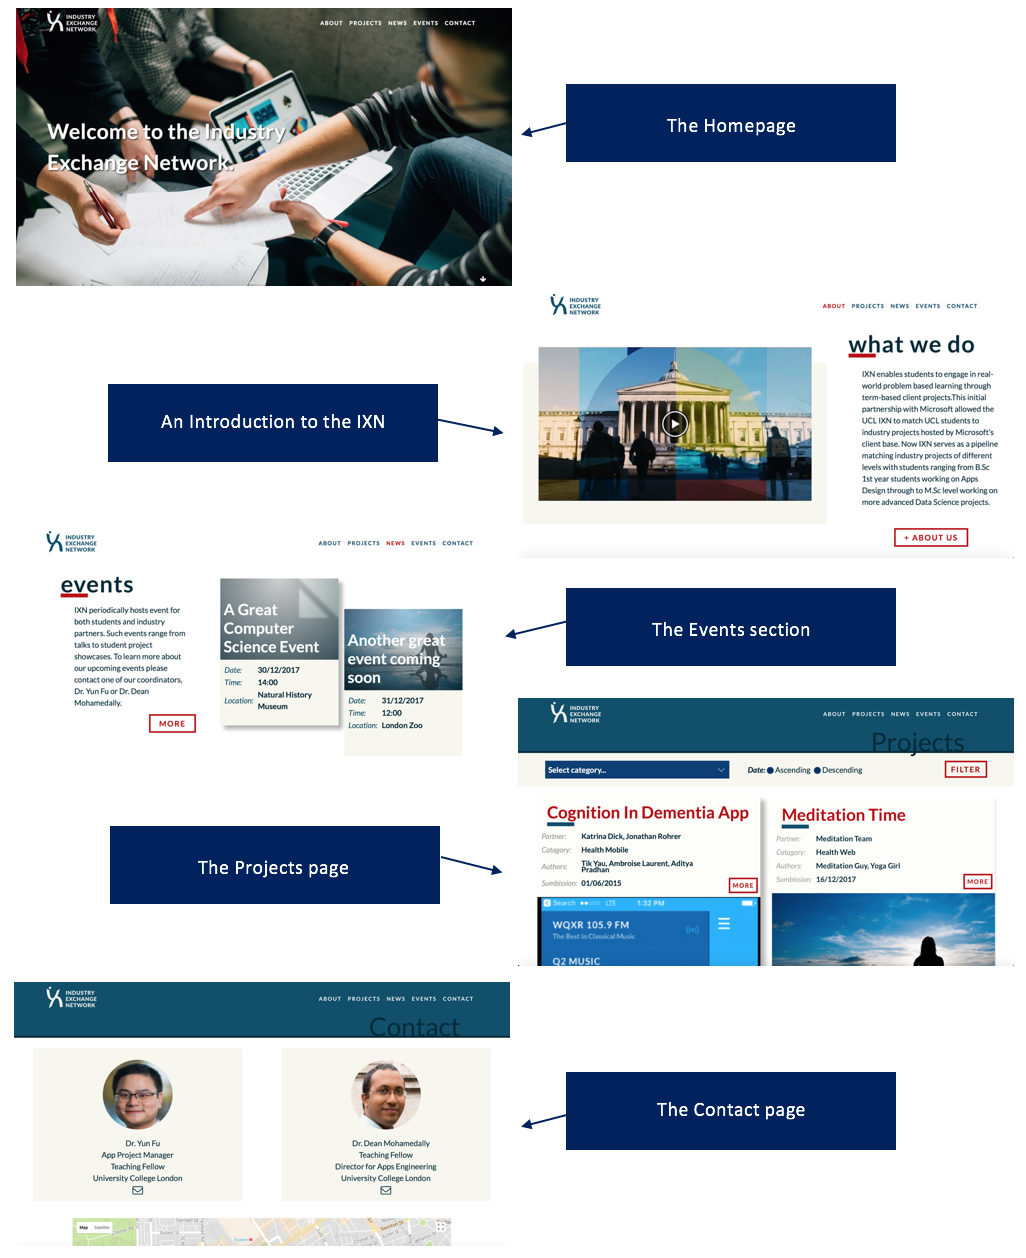
\includegraphics[trim = 0 0 0 0, clip, width=1\textwidth]{ph13.png}
 \end{figure}

\hypertarget{project-management}{%
\section{Project Management}\label{project-management}}

\hypertarget{the-team}{%
\subsection{The Team}\label{the-team}}

\hypertarget{alexander-charles-team-leader}{%
\subsubsection{Alexander Charles (Team
Leader)}\label{alexander-charles-team-leader}}

Alexander obtained a Bachelor of Engineering in Engineering Design
specialising in Aerospace. He has worked with firms including Babcock
International in Marine and Defence and The Manufacturing Technology
Centre (MTC) in Aerospace. Lately, he transitioned into Strategy
Consulting working on advising Telecommunications CEO's on the use of
blockchain technology while at Redshift Strategy. In his spare time,
Alexander has practised web development, building WordPress website for
an array of small clients.

\textbf{Roles:}

\begin{itemize}
\tightlist
\item
  Project Management
\item
  Front End-Development and Optimisation
\item
  Back-end Development and Deployment
\item
  UI Design
\item
  Prototyping
\item
  Report Writing
\end{itemize}

\hypertarget{giovanni-tenderini}{%
\subsubsection{Giovanni Tenderini}\label{giovanni-tenderini}}

Giovanni obtained a Bachelor of Science in Economics and Finance at the
University of Exeter. His work experience includes a Summer Internship
in the Investment Banking division of a Family Office in Milan named CFO
and another internship at Generali Italia insurance sales division. His
overall knowledge of programming is basic. However, he is an expert in
statistical analysis and some related programs.

\textbf{Roles:}

\begin{itemize}
\tightlist
\item
  Testing
\item
  Sketching and Design
\item
  Prototyping
\item
  Final and Weekly Report Writing
\item
  Video Making
\item
  Minimal Front-End Implementation
\end{itemize}

\hypertarget{phoebe-staab}{%
\subsubsection{Phoebe Staab}\label{phoebe-staab}}

A graduate of the BSc Chemistry Programme at University College Dublin,
Phoebe had little to no real programming experience before attending
UCL. She had done a couple of online courses in Java and Python and did
some novice-level statistics programming in R during her undergraduate
degree. Outside of technology-related work, Phoebe has completed several
lab-based research internships at University of Queensland and
University College Dublin.

\textbf{Roles:}

\begin{itemize}
\tightlist
\item
  Prototyping
\item
  Front End-Development
\item
  Report Writing
\item
  Content Creator
\item
  Research
\item
  Minimal Back-end Development
\end{itemize}

\hypertarget{team-coordination}{%
\subsection{Team Coordination}\label{team-coordination}}

In team projects, good organisation is fundamental to effective
collaboration. Productivity tools and workflow management has been key
to the team working efficiently. The key technologies used by the IXN
team included:

\begin{itemize}
\tightlist
\item
  \textbf{Slack:} allowing team members to communicate. Chosen due to
  its ability to share files, track conversations via thread and create
  alerts
\item
  \textbf{Trello:} used as a dashboard to distinguish between work to be
  done, in progress or completed
\item
  \textbf{OneDrive:} used as a cloud sharing tool
\item
  \textbf{GitHub:} used to share code between developers, provide
  version control, manage conflicts and deploy the site to the live
  server. A private repository provided by UCL was used to keep any work
  out of the public domain
\end{itemize}

\hypertarget{scheduling}{%
\subsection{Scheduling}\label{scheduling}}

Work packages were allocated according to each team members' strengths
and weaknesses. Jobs were distributed to optimise team members time
while allowing all individuals to learn. A Gantt chart was used to map
out the timeline of the project to keep tasks on track and manage
deadlines. Figure \ref{gantt}, shows a slimmed down version of the Gantt
chart used.

\begin{landscape}
\begin{figure}[H]
      \centering
      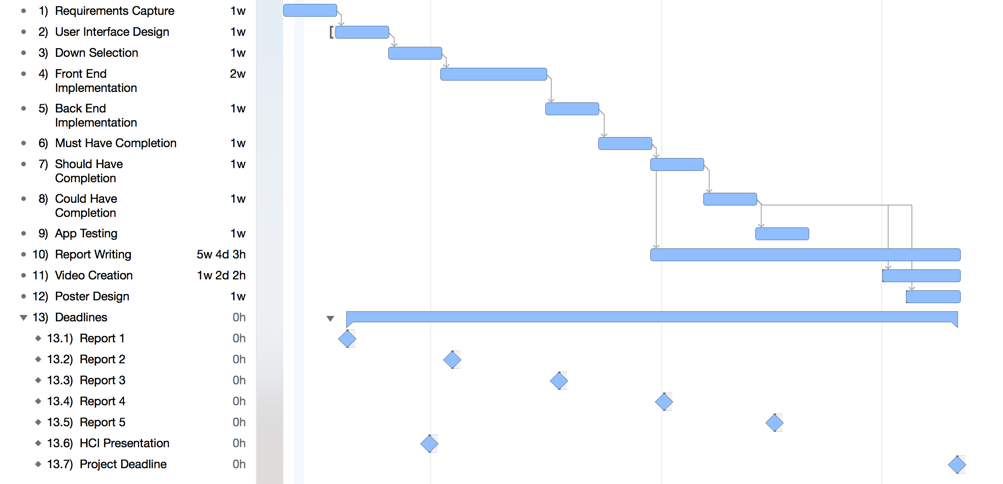
\includegraphics[trim = 0 0 0 0, clip, width=1.3\textwidth]{Picture1.png}
      \caption{Gantt chart where "w" stands for weeks dedicated to the development of each task}
\label{gantt}
 \end{figure}
 \end{landscape}

\newpage

\hypertarget{design-process}{%
\section{Design Process}\label{design-process}}

In order to be able to complete the project to both a high standard an
within a timely manner, a design process was following both process and
agile design methods to reach the projects objectives. The project was
spilt into three phases: \emph{definition, design} and
\emph{development}. Figure \ref{designprocess}, shows an overview of the
projects workflows and a breakdown of the key steps of each phase.

\begin{figure}[H]
\centering
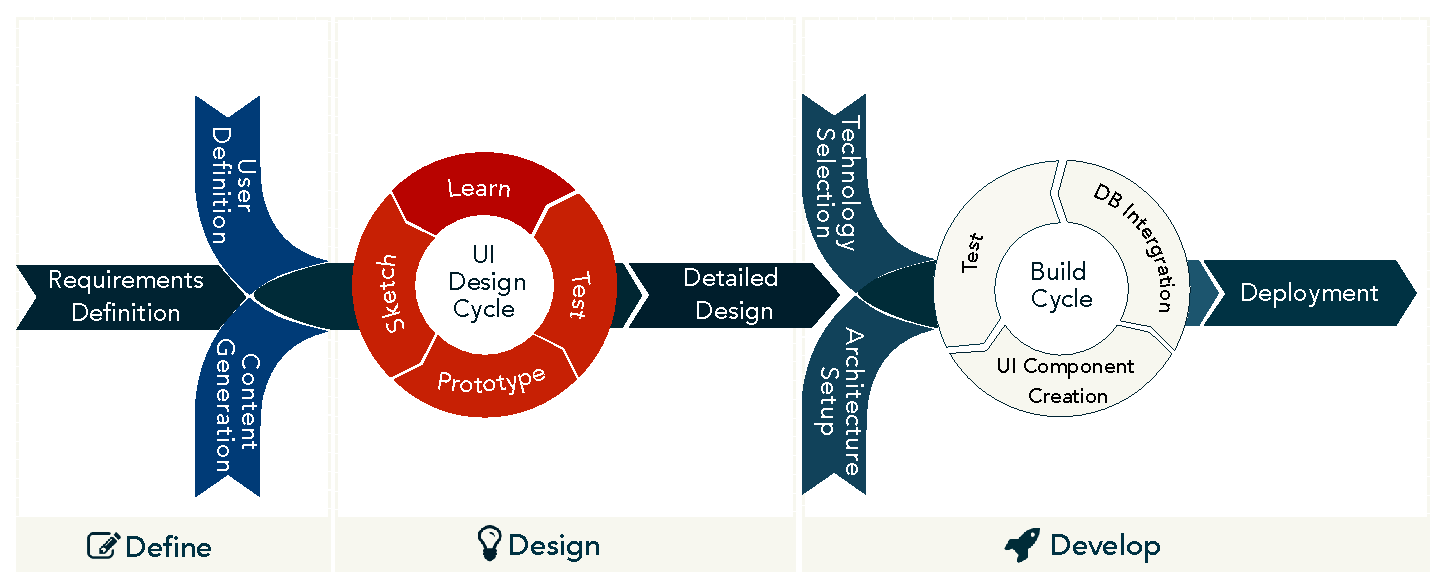
\includegraphics[trim = 0 0 0 0, clip, width=0.98\textwidth]{DesignProcess.eps}
\caption{Diagram illustrating the design process progressing the from the initial briefing to implementation}
\label{designprocess}
\end{figure}

\hypertarget{definition-phase}{%
\subsection{Definition Phase:}\label{definition-phase}}

This phase focused on collecting requirements and defining the
objectives of the project. In order to capture all the information
correctly, several meetings were held with the client these meetings
meetings were used to capture the main features of the site, creating
and organising the content that would be displayed. User research was
then embarked, refining the objectives and content of the site. These
stages all worked towards providing all the prior research required to
begin designing, prototyping and envisioning how the website would
function.

\hypertarget{design-phase}{%
\subsection{Design Phase:}\label{design-phase}}

The design phase applied human computer interaction (HCI) principles in
an agile to approach, to mock up variety of different solutions and
refine the solutions quickly. By following of the process of creating
sketches of different components of the website, whittling these
sketches down to wireframes and prototypes. Solutions could be quickly
tested by the designers, client and user groups providing feedback to
take back and learn upon, improving the overall design of the website
until a rough solution was generated which met both the design
objectives and the met HCI objectives. Spending time before writing any
code was key to making sure the solution was user friendly and visual
meeting one of the key objectives of the project. After rough solution
was created through user interface (UI) design cycle, this was then
padded out and refined creating a static draft of the design which could
be directly copied in the development phase. A large amount of time
could be saved in the development phase of the project by having a
finalised design template to work of which included the typography,
components and the page layouts of the site.

\hypertarget{development-phase}{%
\subsection{Development Phase:}\label{development-phase}}

Development was the final phase of the project. A complete understanding
of how the final product will look and function, based on the research
conducted in the definition phase and the detailed design template in
the design phase meant that all the technology required to required to
implement the solution can be selected. A local development environment
shared amongst all the developers enabled the use of an agile build
cycle, using git to mediate between the different versions. The build
cycle consisted of a developer taking a UI component from the template
and creating the design in code. This would then be connected to the PHP
database using word-press and the tested. Any bugs in either the design
or functionality could then be ironed out through iteration through the
cycle eventually integrating all the components together into the final
site. Once the entire design template was implemented the project could
then be deployed onto the web.

\hypertarget{site-map}{%
\subsection{Site Map}\label{site-map}}

\begin{figure}[H]
      \centering
      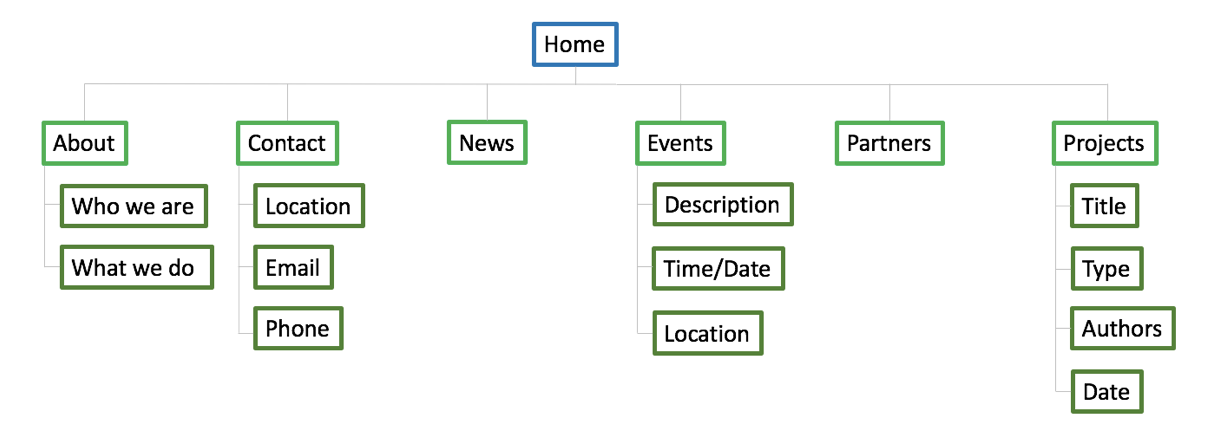
\includegraphics[trim = 0 0 0 0, clip, width=1\textwidth]{ph16.png}
      \caption{Site Map}
      \label{sitemap}
 \end{figure}

\hypertarget{page-flow}{%
\subsection{Page Flow}\label{page-flow}}

\begin{figure}[H]
      \centering
      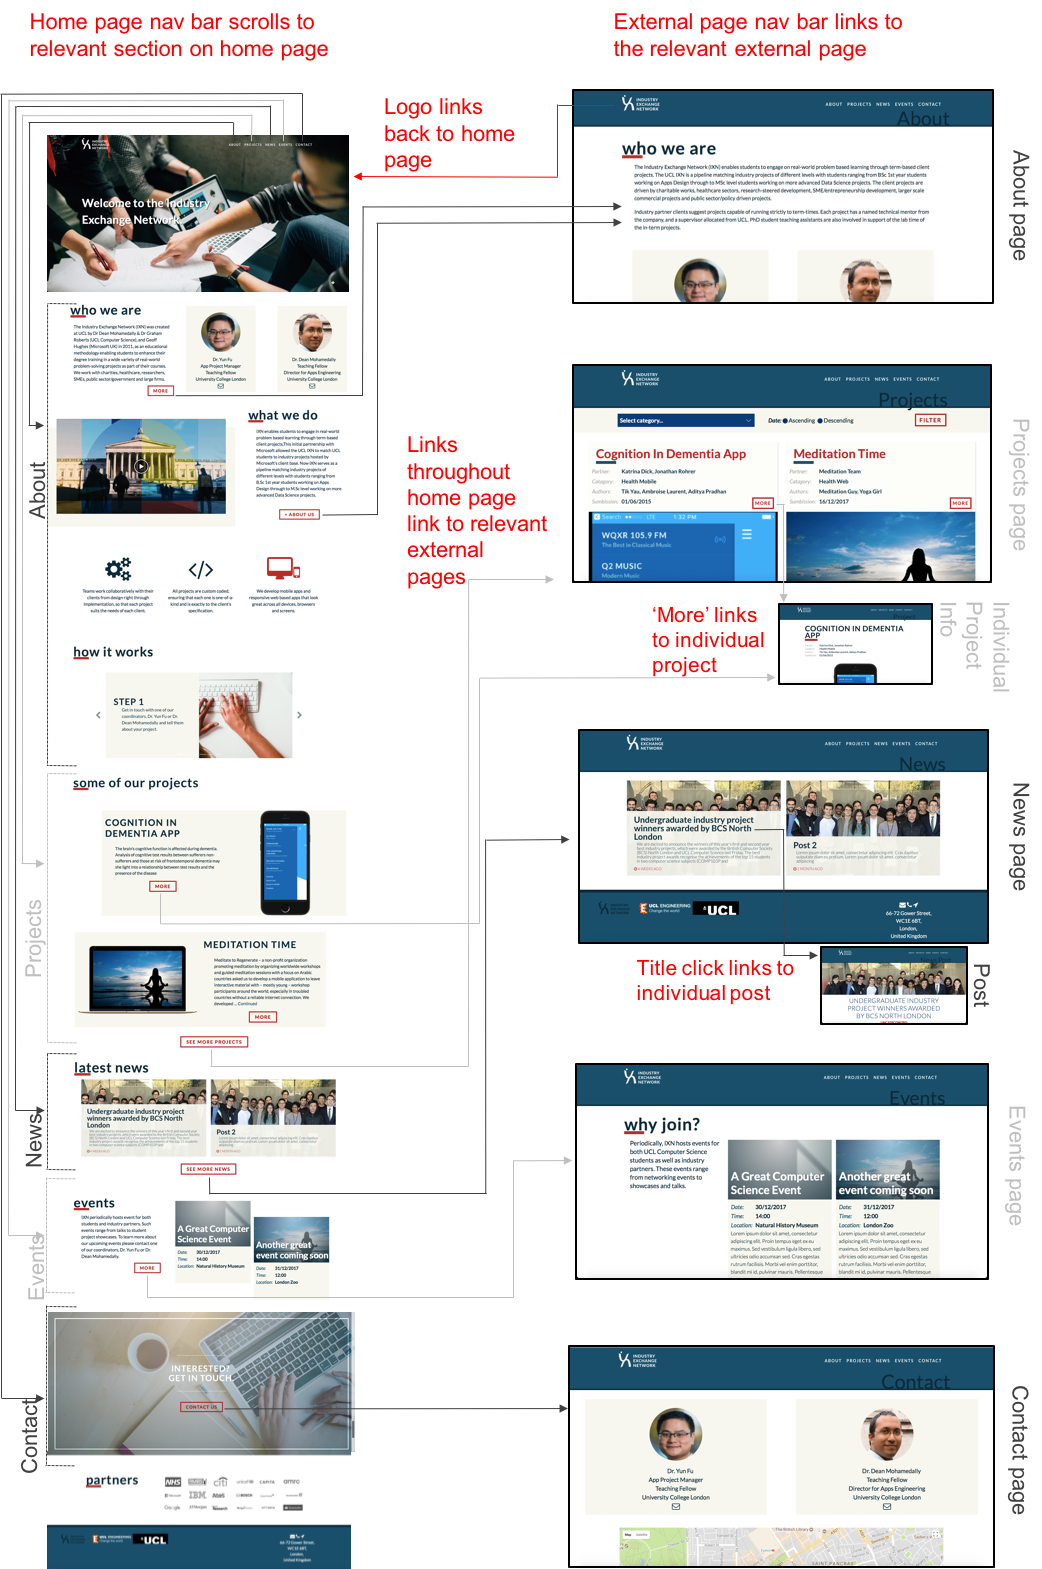
\includegraphics[trim = 0 0 0 0, clip, width=0.82\textwidth]{PageFlow.png}
      \caption{Page Flow}
      \label{pageflow}
 \end{figure}

\newpage

\hypertarget{requirements-definition}{%
\section{Requirements Definition}\label{requirements-definition}}

\hypertarget{client-requirements}{%
\subsection{Client Requirements}\label{client-requirements}}

The primary requirements of the IXN website were highlighted in the
first meeting with Dr Yun Fu. The client explained that the aim of the
Industry Exchange Network website is to encourage new industry partners
to join the programme. Therefore, new website had to be a high quality
example of what the department is capable of and the following features
were required by the client:

\begin{itemize}
\tightlist
\item
  High quality and professional design
\item
  Fully responsive website
\item
  Content management system to allow the Administrator to update the
  website without touching code
\item
  Separate pages for Events, News, Contact and Featured Projects.
\item
  A navigation bar always present at the top of the website
\end{itemize}

\hypertarget{types-of-requirements}{%
\subsection{Types of Requirements}\label{types-of-requirements}}

There are two types of requirements in web development: functional and
non-functional. The former define specific tasks and activities that the
project must be able to perform. The latter outline the way that a
system operates and strongly related to the architecture of the system
\cite{g5}. Due to the nature of a website used to showcase projects,
most of the requirements fall under the functional category,
nonetheless, all of the most important requirements are listed below:

\hypertarget{functional-requirements}{%
\subsubsection{Functional Requirements}\label{functional-requirements}}

\begin{itemize}
\tightlist
\item
  Professional and highly polished design
\item
  Displaying news and events related to the Industry Exchange Network
\item
  Showcasing projects made by the CS department through images and
  videos
\item
  A navigation bar which is always present at the top of the webpage
\item
  Displaying partners of the IXN
\item
  Project Sorting tool
\end{itemize}

\hypertarget{non-functional-requirements}{%
\subsubsection{Non-functional
Requirements}\label{non-functional-requirements}}

\begin{itemize}
\tightlist
\item
  Content Management System allows and admin to update the website
  without having to modify the code directly.
\item
  Scalability when inserting new projects, news and events
\end{itemize}

\hypertarget{moscow}{%
\subsection{MoSCoW}\label{moscow}}

To distinguish between Must-Have requirements, Should and Could-Haves
the team used a MoSCoW analysis framework \cite{g4}. The tool was
constructed by combining statistics extracted from surveys, Client
Requirements, Personas and Use Cases. A well developed MoSCoW
facilitates the implementation and design of a project by streamlining
the creation and implementation processes. The MoSCoW of the IXN project
is displayed below:

\newpage

\begin{landscape}
\begin{table}[H]
      \centering
      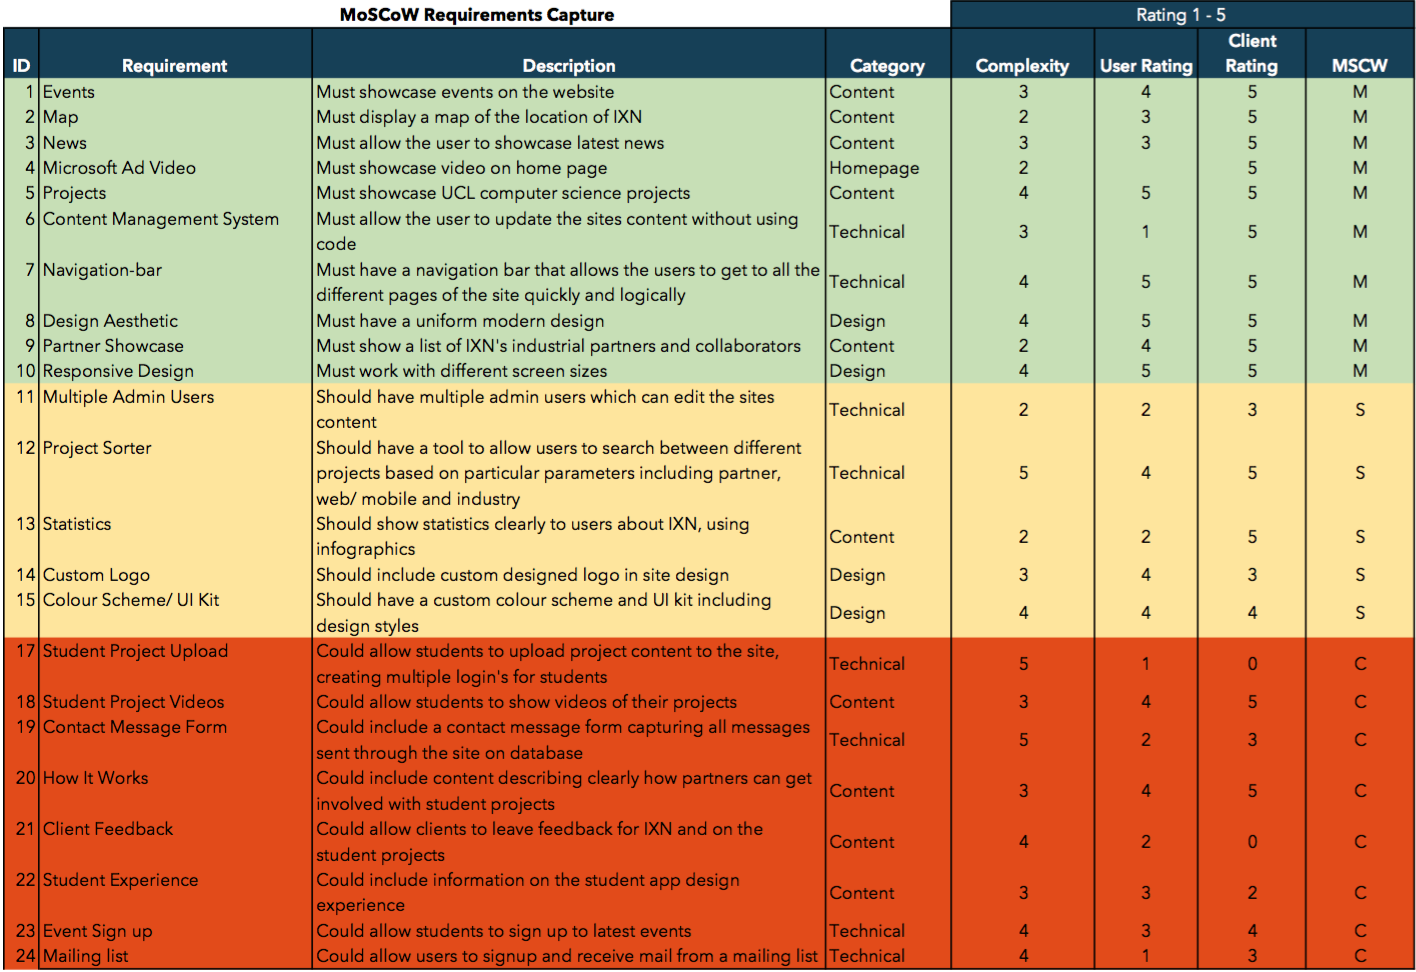
\includegraphics[trim = 0 0 0 0, clip, width=1.3\textwidth]{ph2.png}
      \caption{MoSCoW framework applied to IXN website requirements}
 \end{table}
 \end{landscape}

\hypertarget{user-definition}{%
\section{User Definition}\label{user-definition}}

\hypertarget{round-one-user-feedback}{%
\subsection{Round One User Feedback}\label{round-one-user-feedback}}

Evaluation is concerned with gathering data regarding the usability of a
design or a product by a specified group of users within a specified
environment or work context. The first round of user surveys was taken
based on sketches in order to assess essential site content. The results
were used to inform a MoSCoW, storyboards, and subsequent sketches. The
results of the survey are outlined below:

\begin{table}[H]
      \centering
      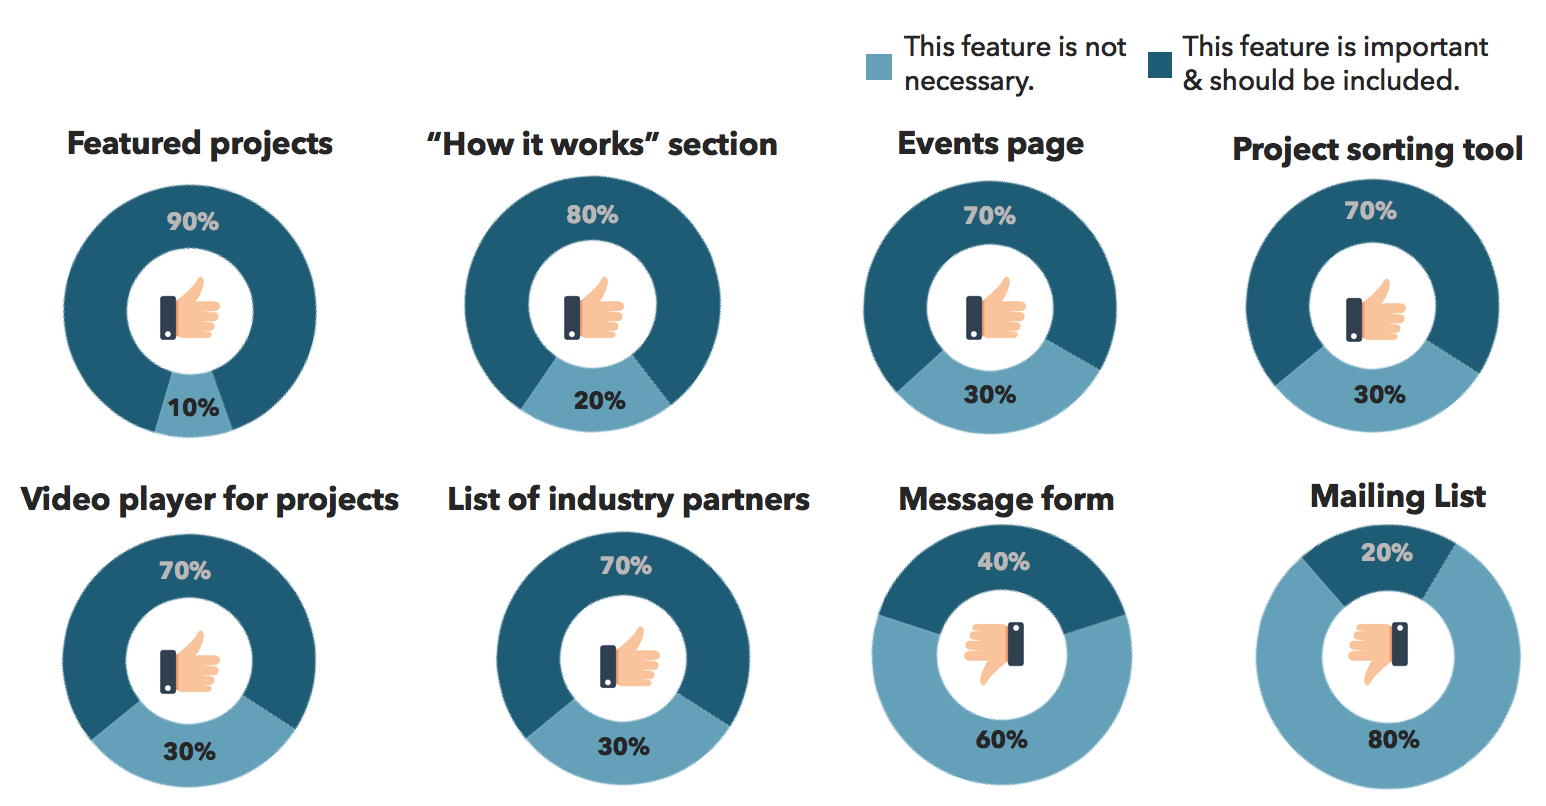
\includegraphics[trim = 0 0 0 0, clip, width=0.7\textwidth]{ph3.png}
      \caption{IXN network round one User Feedback result summary}
\label{userfeedback}
 \end{table}

As can be seen, the features which were given highest importance were
project-related features and IXN information-related features.
\ref{userfeedback} In addition to these content-related attributes, it
also became evident that the design-quality would be of utmost
importance, given that the site is meant to attract prospective industry
partners.

\hypertarget{related-research}{%
\subsection{Related Research}\label{related-research}}

Related research was highly important due to the red tape imposed by
regulations at UCL. External sources were used to understand the type of
audience that the website would appeal to and what level of digital
ability the users typical would have. The image below outlines the
outcomes of such research:

\begin{table}[H]
      \centering
      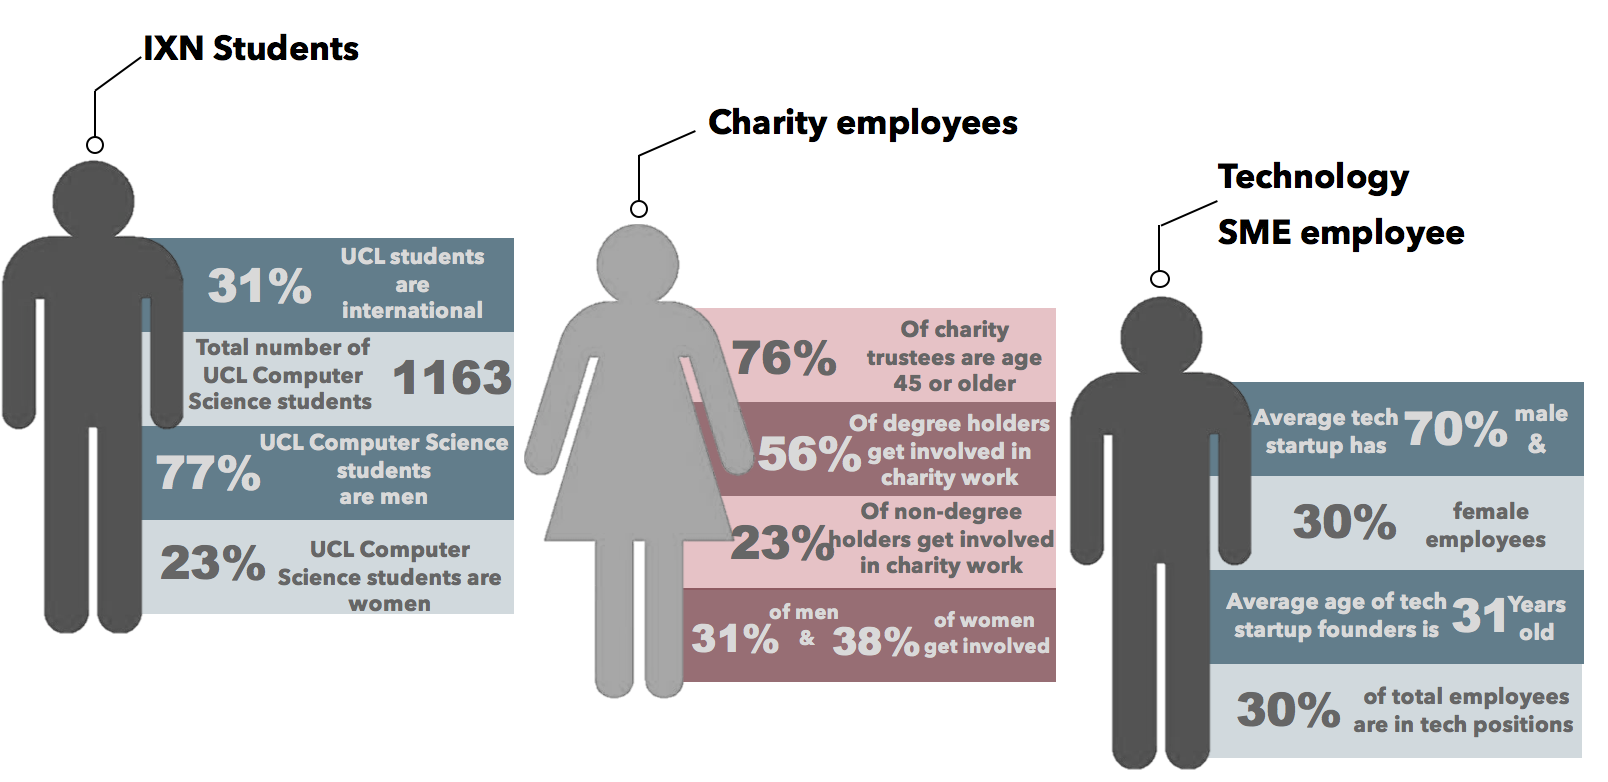
\includegraphics[trim = 0 0 0 0, clip, width=0.7\textwidth]{p21.png}
      \caption{Summarized statistics extracted from the readings explaied below}
 \end{table}

Data providing a fuller picture of the demographics of IXN Students was
found primarily using UCL student statistics \cite{ps1}. This
information was provided on the UCL website. It was determined that the
IXN student audience is typically British and male. This evidence helped
us develop a data-driven persona. The client indicated that this is not
a target-user, but never the less, user research determined that UCL IXN
students would be an audience regardless of the website's intent since
they would like to see their work, the work of other students, and
possible industry partners.

The client's target audience for the IXN site was potential and current
partners. Based on the assigned projects for GC02 during the current
term, the partners tend to be from technology companies and charity
institutions.

Research was done on the demographics of a typical charity volunteer/
employee in the United Kingdom using sources such as The Charity
Commission \cite{ps2} and National Council for Voluntary Organisations
\cite{ps3}. Based on worked published from these organisations, it was
determined that the typical charity employee is aged 45 or older and
usually holds a degree. A persona and use-case was developed regarding
this data. This data also indicated that the site should be streamlined
and simple without confusion on how to navigate through different pages.

In order to obtain a profile for a technology employee, sources such as
the Atlantic \cite{ps4} and The Harvard business review \cite{ps5} were
utilised. The research indicated that employees at such businesses are
typically males in their early to mid-thirties. This data was, again,
used to inform a persona/use-case scenario. It was determined that this
type of user is typically technology-proficient and that the site should
reflect the high calibre of technical capability of IXN students.

\hypertarget{limitations}{%
\subsection{Limitations}\label{limitations}}

The main limitations were imposed by the HCI department which did not
allow surveys to be taken from those other than immediate family members
or UCL CS students. Fortunately, in the case of the Industrial Exchange
Network, UCL Computer Science students account for a high percentage of
users. Had more time and leniency been given for user research, a
broader audience could have been surveyed resulting in a more in-depth
study of user requirements. Having a budget to dedicate to research
could have also helped to obtain more statistically significant results.
For example, questionnaires could have been sponsored to attract a
larger public to complete them.

\hypertarget{users-and-personas}{%
\subsection{Users and personas}\label{users-and-personas}}

Based on client specification and demographics research, 5 personas were
created to gain understanding of the end user of the product. Please
refer to Figure ``X'' in the Appendix for detailed personas. The two
main user categories that were focused on were: ​

• Technology industry employees: ​ - Digital Native Users who have got
strong tech background​ - Look for a business opportunity​ - High
expectations from design and quality of website​ - The platform has to
appear professional for them to be incentivised to join IXN​.

The main design principles were considered for this specific persona
were: ​ consistency: essential for a professional looking website​
affordance: for an intuitive interaction with the platform. ​

\begin{table}[H]
      \centering
      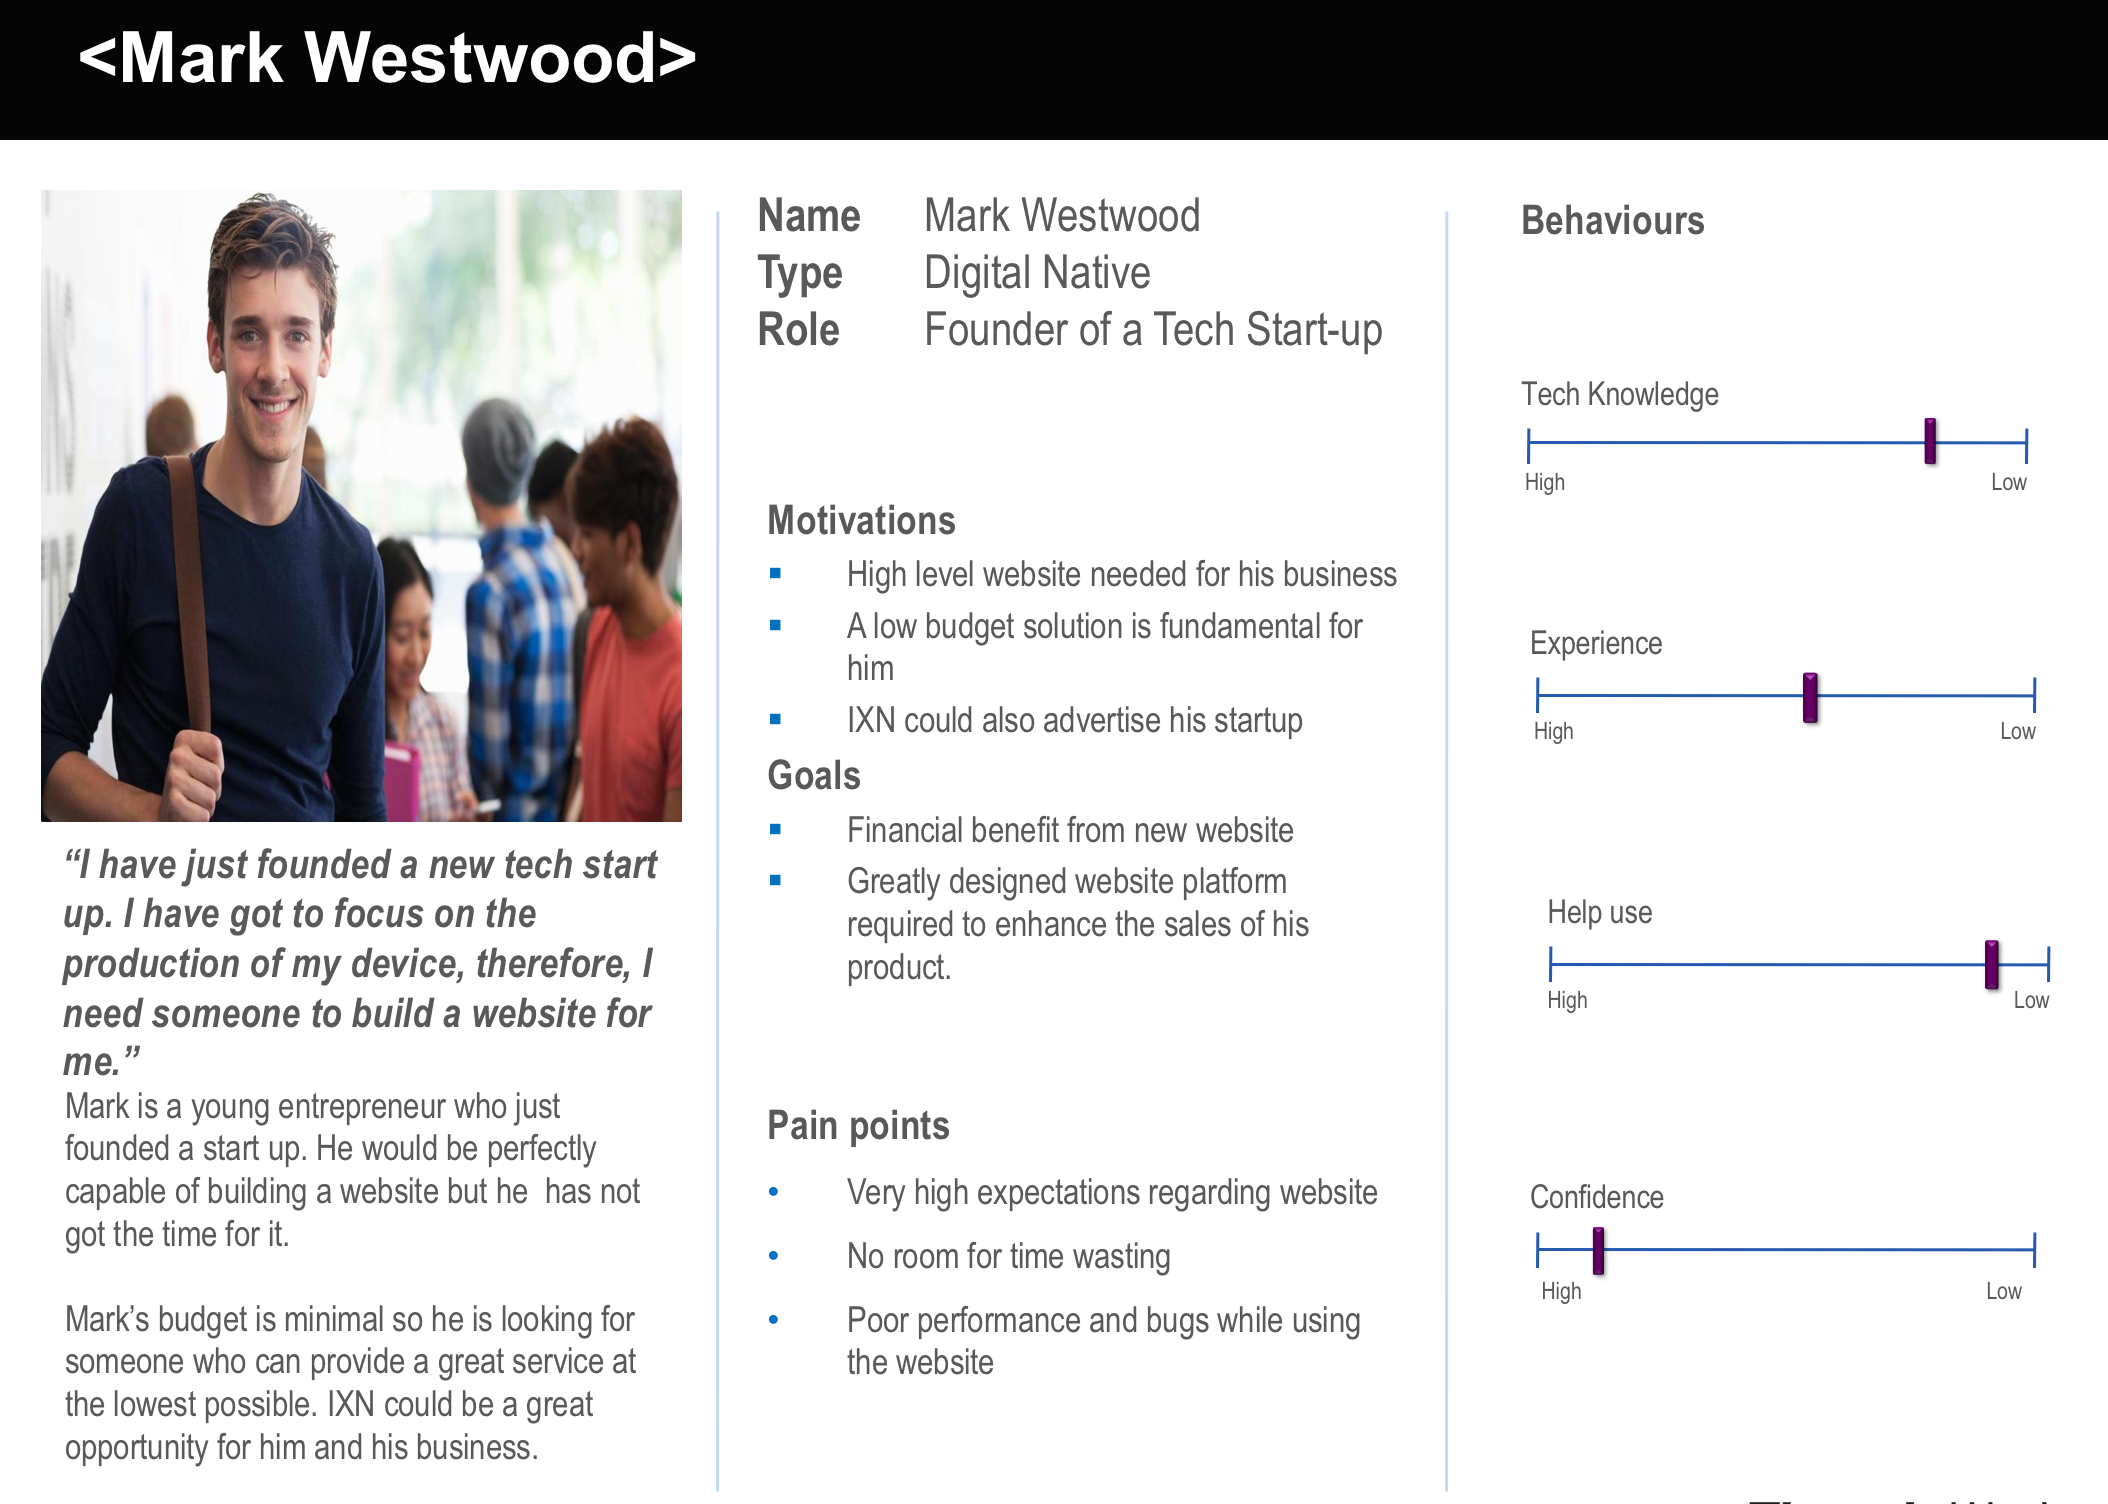
\includegraphics[trim = 0 0 0 0, clip, width=0.7\textwidth]{ph1.png}
      \caption{SME Tech Enterprise Owner}
\end{table}

• UCL Computer Science Students: ​ - Highly trained digital users​ -
They require the projects they have worked on to be very visible​ -
Expect to be well represented by the design of the website​ - They
desire the platform to be as entertaining as possible. ​

The main design principle was considered for this specific persona was:
​ visibility: especially in relation to how the projects are showcased.
​

\begin{table}[H]
      \centering
      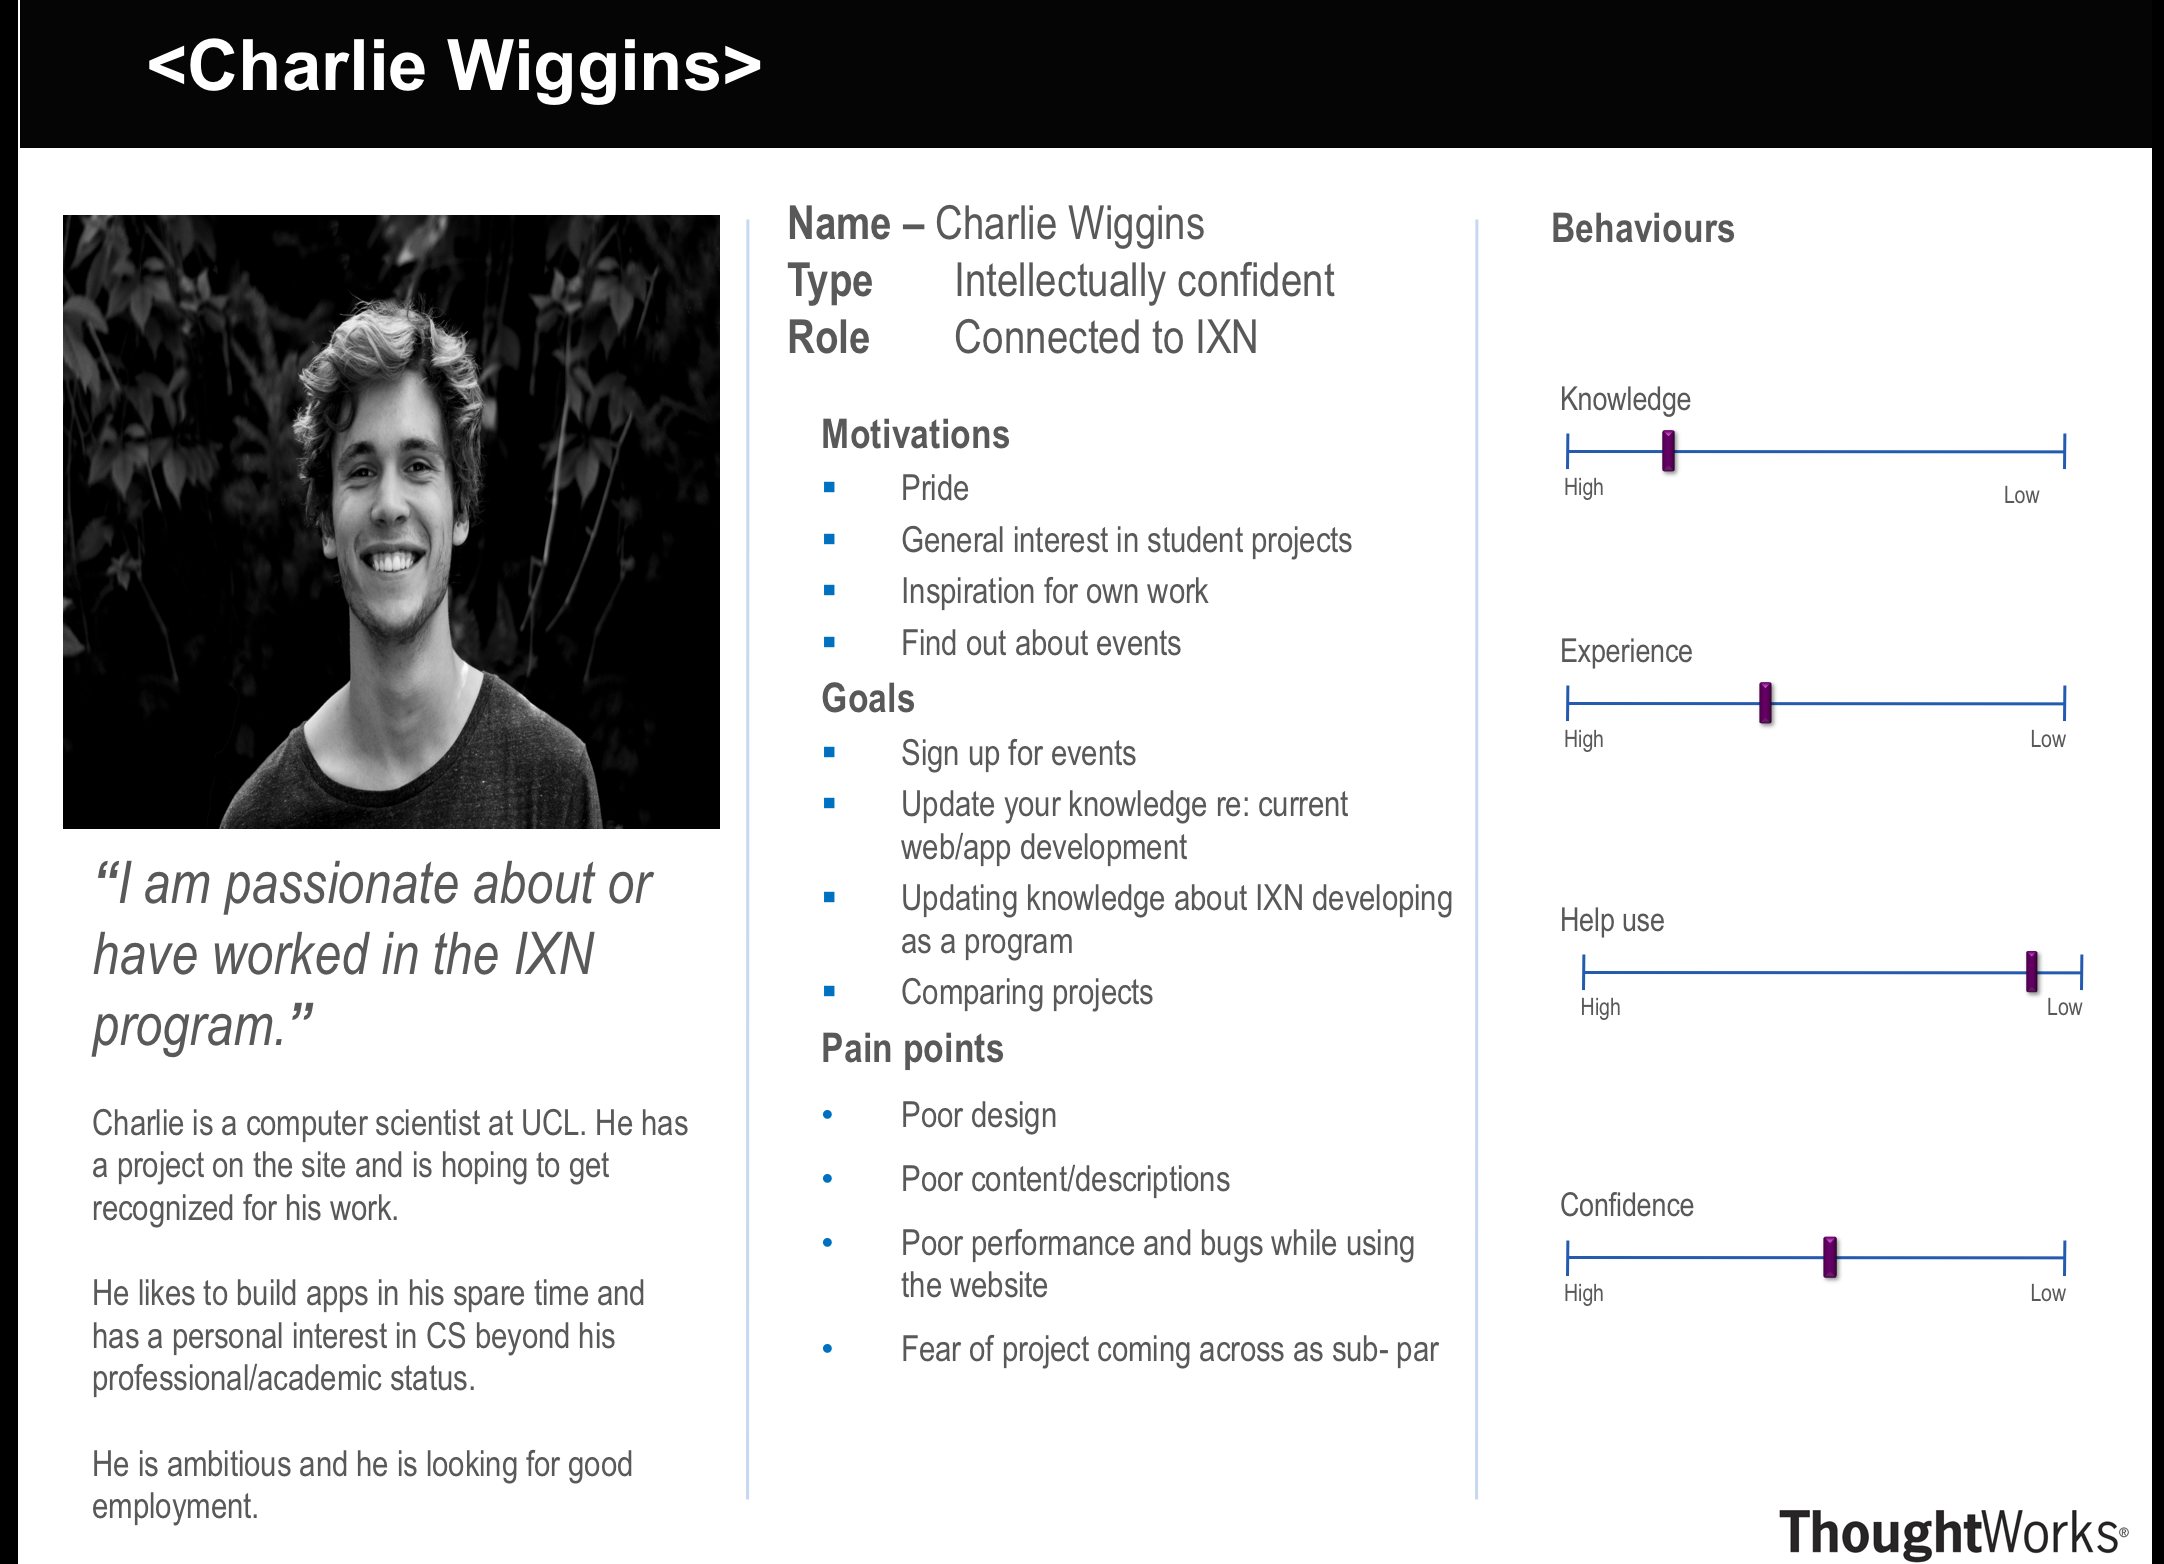
\includegraphics[trim = 0 0 0 0, clip, width=0.7\textwidth]{persona1.png}
      \caption{UCL Computer Science Student}
\end{table}

Use Cases

Use cases were constructed to represent the standard user navigation and
interaction with the platform needed to accomplish a given task
\cite{g3}. These were useful in shaping the development and design of
the website, and facilitating the interaction between the website and
its users. In the case of the IXN website the role of the administrator
was also taken into account.

\begin{table}[H]
      \centering
      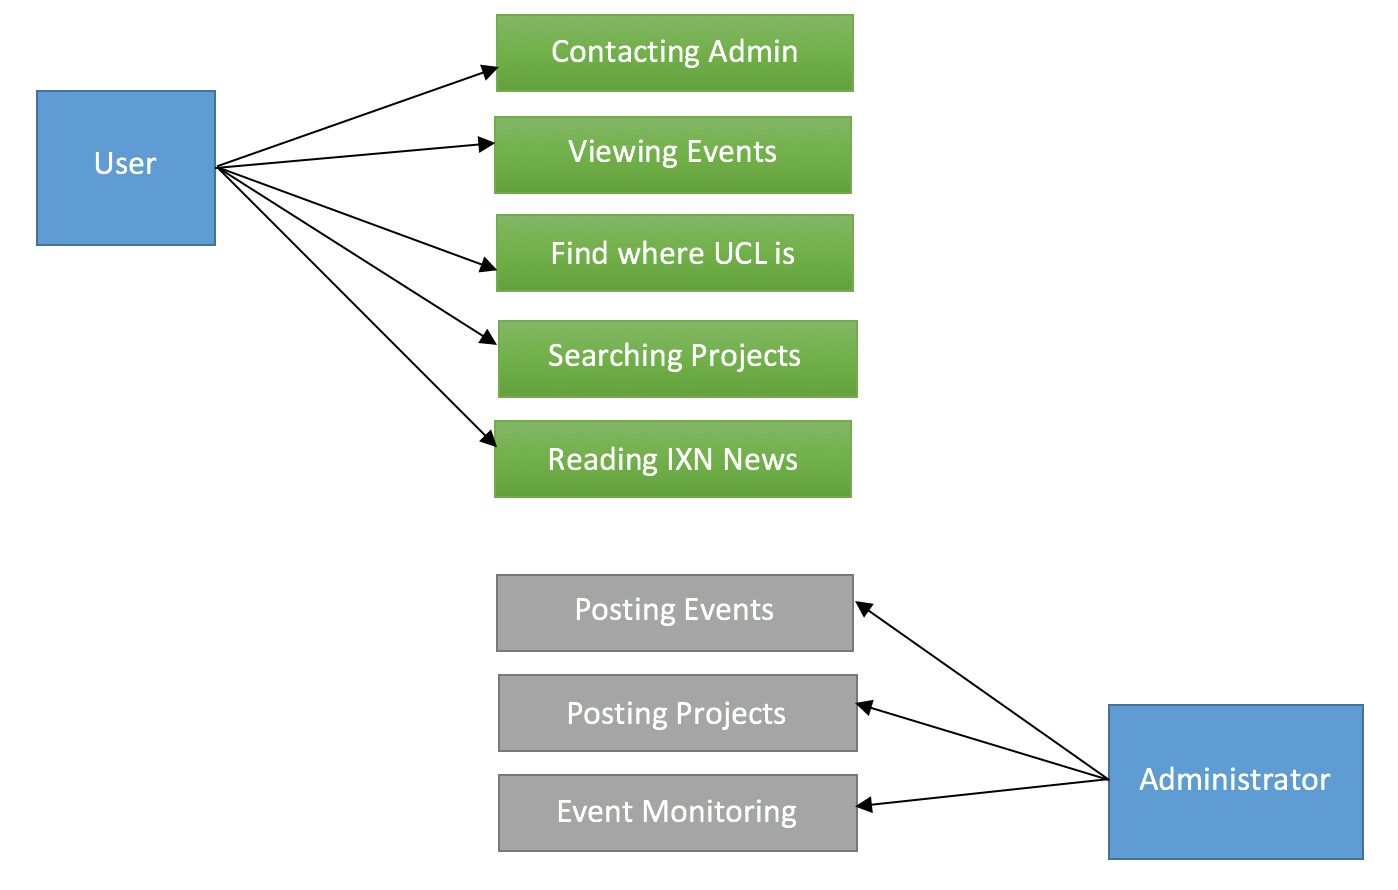
\includegraphics[trim = 0 0 0 0, clip, width=0.7\textwidth]{ph9.png}
      \caption{Use case graph}
\end{table}

An outline of the use cases can be found below. This is essentially a
list of the actions realated to the Must and Should sections of the
MoSCoW. To avoid repetition, the main routes (in bold) have been
outlined in detail.

\begin{table}[H]
      \centering
      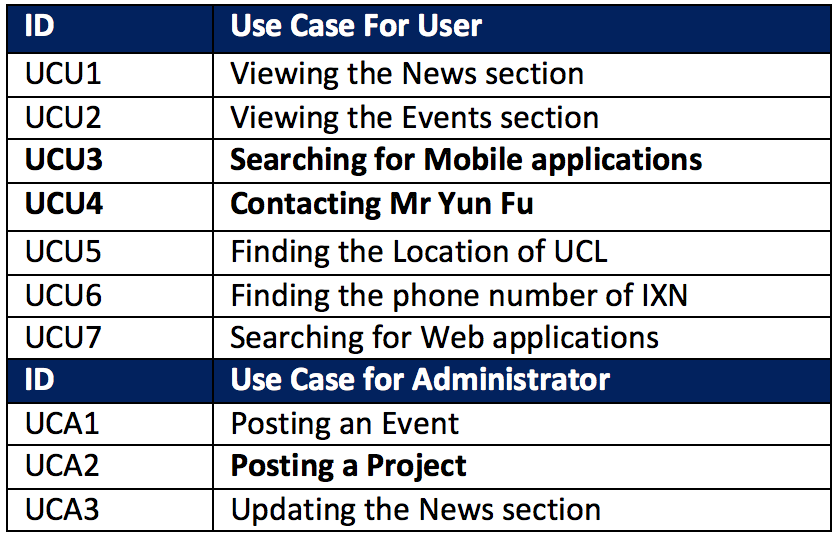
\includegraphics[trim = 0 0 0 0, clip, width=0.7\textwidth]{ph10.png}
      \caption{Use case list}
 \end{table}

\begin{table}[H]
      \centering
      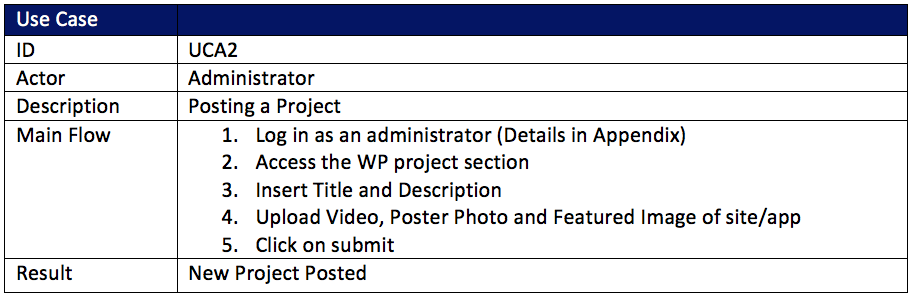
\includegraphics[trim = 0 0 0 0, clip, width=0.7\textwidth]{UCA2.png}
      \caption{Detailed UCA2}
 \end{table}

\begin{table}[H]
      \centering
      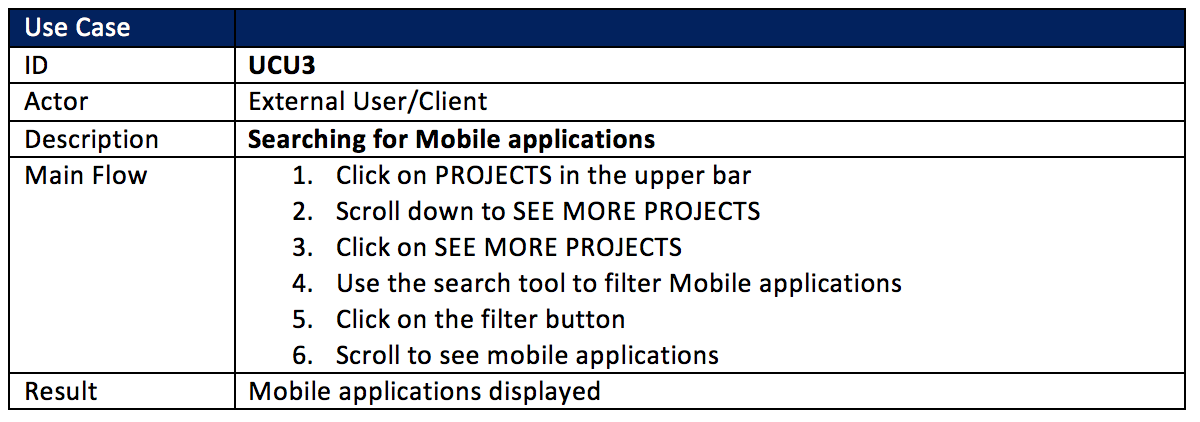
\includegraphics[trim = 0 0 0 0, clip, width=0.7\textwidth]{ph12.png}
      \caption{Detailed UCU3}
 \end{table}

\begin{table}[H]
      \centering
      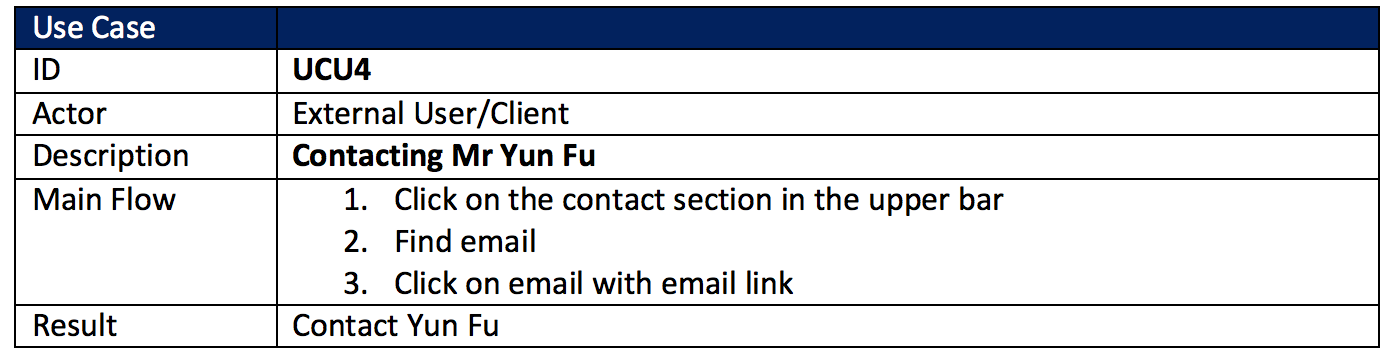
\includegraphics[trim = 0 0 0 0, clip, width=0.7\textwidth]{ph11.png}
      \caption{Detailed UCU4}
 \end{table}

\hypertarget{user-interface-design}{%
\section{User Interface Design}\label{user-interface-design}}

\hypertarget{ui-design-cycle}{%
\subsection{UI Design Cycle}\label{ui-design-cycle}}

After the initial debrief with the client, describing what the Industry
exchange Network does and the primary website requirements, the HCI
design process began. Initial research into competing solutions revealed
that there was no exact equivalent to IXN. However, there were specific
features of similar sites that would later inspire IXN content, such as
``How to use'' sections, ``Events'' sections and prominent placement of
industry links.

Based on initial research including competing solutions, initial user
surveys and client meetings, a shortlist of potential user types was
obtained and was used to inform several personas and use-case scenarios.
Throughout the entire research process, iterations of hand-drawn
sketches were made in an attempt to hone in on an ideal data-driven
design. Additionally, storyboards were made to outline specific user
experiences.

After the second round of user feedback, a MoSCow requirements table was
defined in order to inform several generations of wireframes.
Down-selection of such wireframes gave way to an initial prototype which
was then scrutinised via Heuristic and Think-Aloud user evaluation. The
final prototype that inspired the IXN website design was developed over
several iterations based on all of the data obtained during the HCI
portion of the course.

\begin{table}[H]
\centering
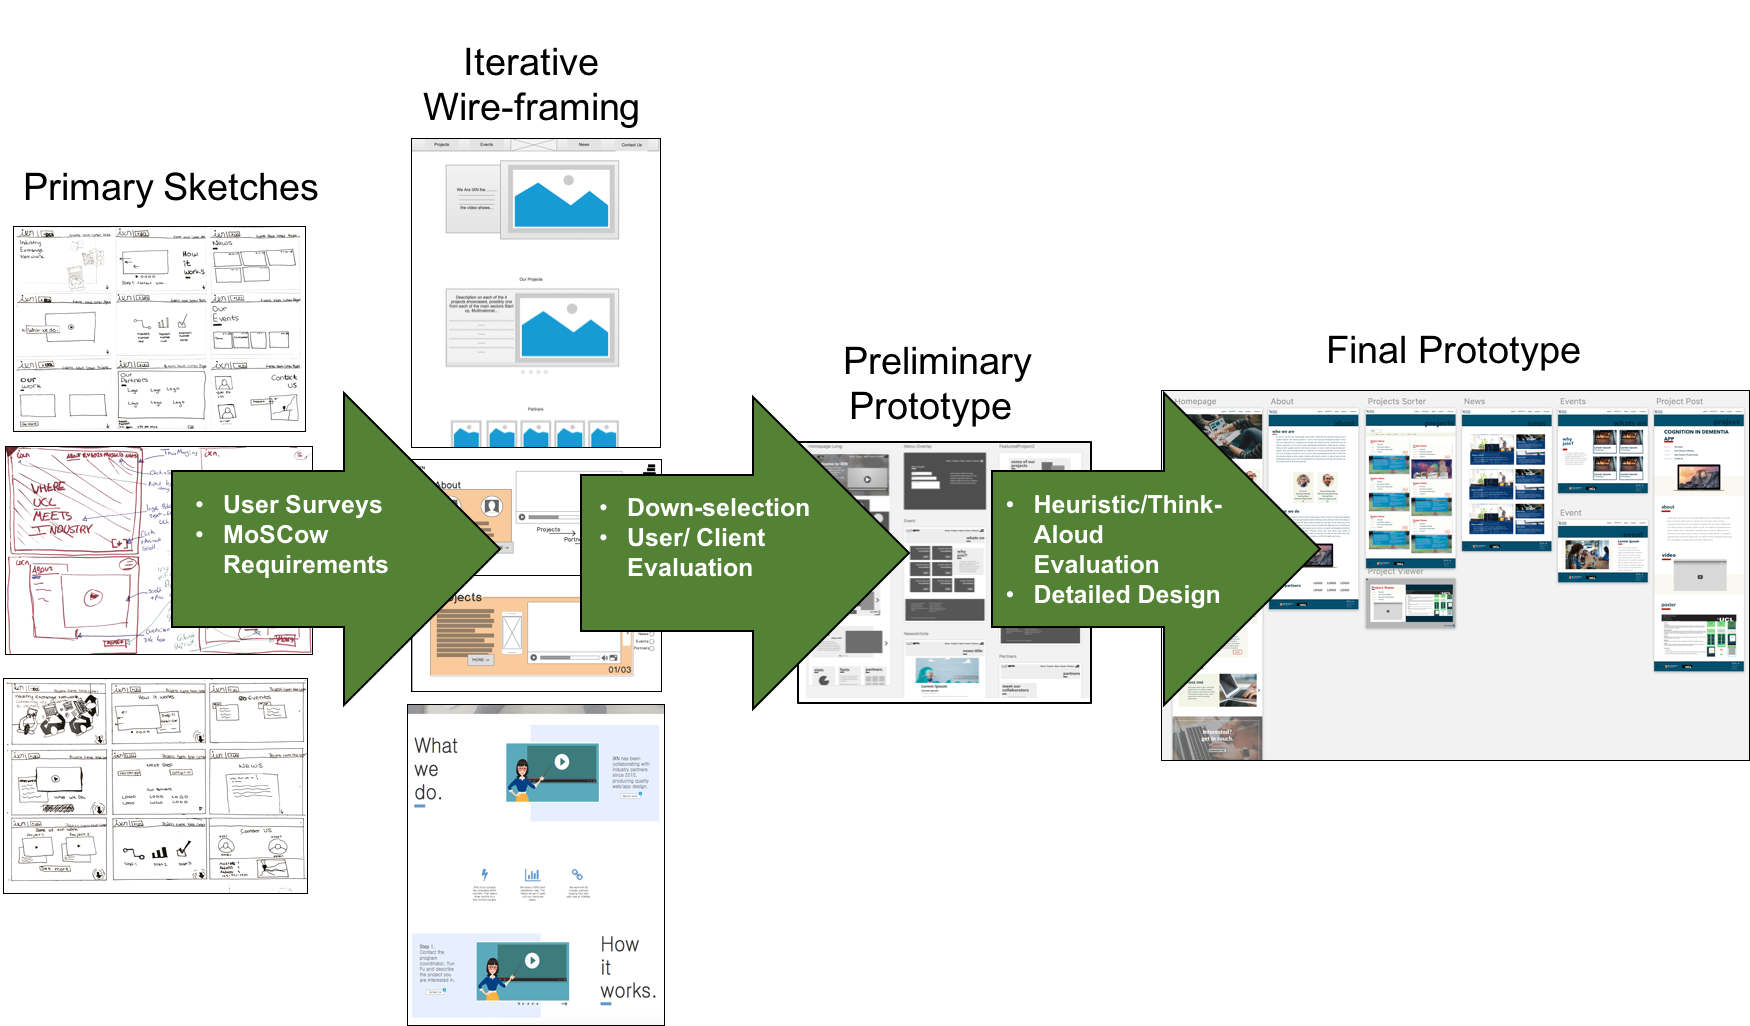
\includegraphics[trim = 0 0 0 0, clip, width=0.98\textwidth]{UIDesign.png}
\caption{UI Design Cycle}
\label{UIDesign}
\end{table}

Various tools were used to turn handmade sketches into a final
prototype. The table below explains which methods have been used and the
reason they have been chosen:

\begin{table}[H]
      \centering
      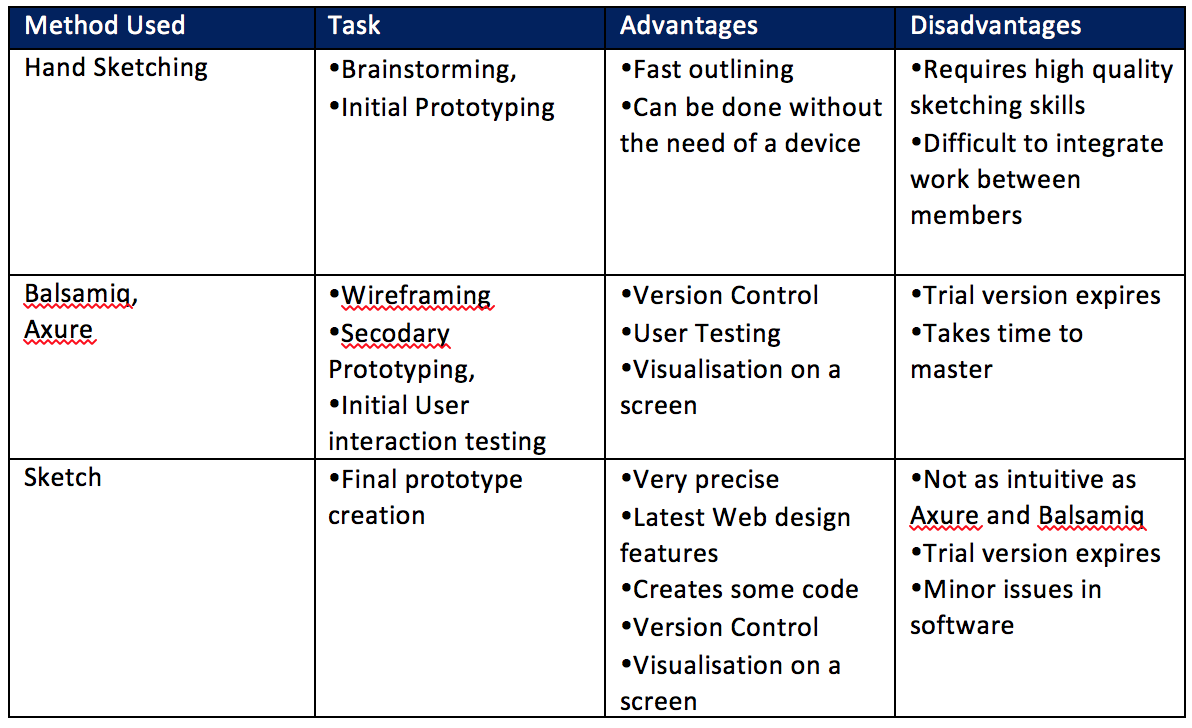
\includegraphics[trim = 0 0 0 0, clip, width=0.98\textwidth]{ph19.png}
      \caption{Prototyping methods and tools used}
 \end{table}

\hypertarget{detailed-design}{%
\subsection{Detailed Design}\label{detailed-design}}

Sketch was used to make the final prototype, which was then employed
directly in front-end development. Each member of the team took
responsibility for designing both the web and mobile views for
particular components of the IXN site. In Sketch, both Symbols and UI
Components sheets were made, housing key design elements of the site in
order to avoid redundancy and maintain consistency throughout the site.
Sketch's ability to produce exportable CSS code based on prototype
design elements made the tool particularly useful during the
implementation stage of development. An example would be the IXN
website's section headings. A symbol was created in order to maintain a
consistent design of this feature for all of the sections on the
homepage and throughout the external pages.

After components were individually designed, the team came together to
ensure a cohesive flow was maintained throughout the site. Small tweaks
were made to individual components in order to ensure a consistent user
experience across every part of the IXN website. After this
collaborative effort concluded, front-end development commenced.

\begin{figure}[H]
\centering
\includegraphics[trim = 0 0 0 0, clip, width=0.98\textwidth]{SketchDD.png}
\caption{Diagram showing an overview of the final detailed design Sketch template}
\label{sketchdd}
\end{figure}

\newpage

\hypertarget{technical-research}{%
\section{Technical Research}\label{technical-research}}

\hypertarget{content-management-system}{%
\subsection{Content Management System}\label{content-management-system}}

A content management system (CMS) is a piece of software which provides
a level of automation for the tasks required to manage content
efficiently. It is usually server-based, interacting with content stored
in a repository; which can be located on the same server \cite{p1}. In
web development, the ultimate purpose of such tools is to allow an
administrative user to edit the content on a website without having to
append code files directly.

The CMS used for the IXN project was WordPress. There are other free,
open-source CMS options, such as Drupal or Joomla, but WordPress was
selected due to a few critical advantages.These can be boiled down to:

\begin{enumerate}

\tightlist
\item
  Better support options and availability
\item
  Superior access to themes and add-ons
\item
  Easy website maintenance.
\end{enumerate}

\hypertarget{support-options-and-availability}{%
\subsubsection{Support Options and
Availability~}\label{support-options-and-availability}}

WordPress support is available on a plethora of developer channels for
web developers and beginners alike on a myriad of platforms. These
include docs, handbooks, codex, Slack channels and Stack Exchange to
name a few. Being the most popular CMS, there are entire websites
dedicated to supporting in addition to thousands of online tutorials.
Unlike WordPress, finding expert support for Joomla or Drupal is more
difficult. All of the platforms provide extensive primary source
documentation, but~because of WordPress's popularity, it outshines its
competitors as far as ease of access to efficient troubleshooting.~

\hypertarget{access-to-themes-and-add-ons}{%
\subsubsection{Access to Themes and
Add-ons~}\label{access-to-themes-and-add-ons}}

While Drupal and Joomla also both offer themes and add-ons, the access
and variety are not comparable to WordPress, which offers around 40,000
additional plugins. In Joomla, there is a feature that allows users to
install extensions. However, to access a template, a user would still
have to manually search templates and then install them by adding their
URL, more arduous than WordPress streamlined process using the
dashboard. Worse still, Drupal users have to exit their site, search for
a specific module or theme, find a zip file URL and submit the URL to
the Modules or Themes page to install them.~

Not only does WordPress take minutes to install, but also the dashboard
interface after the install is simple and easy to navigate \cite{p3}.
This is especially useful if you are developing a simple site for a
client and they want to be able to manage and modify the site's content
easily. Updating Wordpress is a seamless process often requiring no
developer interaction. It should also be mentioned that To increase
accessibility, WordPress offers a mobile app that users can download to
monitor and update their site. Joomla's post-install panel less
intuitive, partly due to offering many more features out of the box
\cite{p2}. Seasoned web developers may~prefer this, but for simplicity,
WordPress wins out. Drupal offers users \emph{`distributions'},
particular to the type of site that they want to develop. This could be
a bit confusing for beginners. Finally, Drupal's updates can require
developer knowledge \cite{p4}.

\hypertarget{roots-technology-stack-sage-bedrock-and-trellis}{%
\subsection{Roots Technology Stack: Sage, Bedrock and
Trellis}\label{roots-technology-stack-sage-bedrock-and-trellis}}

Traditionally, Wordpress app development and deployment involves
installing Apache, My SQL and PHP locally, often installed using
software such and MAMP or WAMP. Servers (particularly shared hosting
providers) often provide WordPress installs using a one-click install
method. This prevents the developer having to configure installation and
setup of the production server remotely but limits files to be uploaded
via File Transfer Protocol (FTP) only. This method has many limitations
and is highly unsuitable for professional website development. Some of
the limitations include:

\begin{enumerate}

\tightlist
\item
  No relationship between local and production files creating
  duplication of work
\item
  Databases between local and production will be different and hard to
  sync across
\item
  If an error occurs when updating production files, the entire
  production site can be corrupted suspending the websites service to
  users
\item
  FTP sites can be very slow to load and update
\item
  Plugins and backend changes have to be completed through the control
  panel and no WP-CLI access is provided \cite{p13}
\end{enumerate}

The Root's open source technologies instead provide a different more and
superior approach to Wordpress app development; through creating
development and production environments, ensuring that production
environments server match the development virtual machine precisely.

To illustrate; after creating a new theme or plugin for a Wordpress site
on a local server, it is time to deploy. The Sage starter theme offer
out of the box code optimisation technology which requires compiling.
Through typing a single line of code a developer can install or update
all the correct version of the plugin on the production site, compile
assets, update the theme on the remote server, and then ensure the
plugin has been activated on the production site while maintaining the
database between the local and development sites. Through using Sage,
Bedrock and Trellis in unison, the process of developing, testing and
deploying can be reduced to a fraction of the time while the site can be
fully optimised and remain online and stable. The following subsections
give more detail to the three Roots technologies:

\hypertarget{bedrock}{%
\subsubsection{Bedrock}\label{bedrock}}

Bedrock is a modern WordPress stack that brings more automation to web
development and site maintenance and does so using a better folder
structure, see Figure \ref{bedrockfolder}. It uses PHP \emph{.dotenv}
for environment variables, which are part of the twelve-factor app
\cite{p6}, a methodology created by Heroku for building web
apps\cite{p5}. The main goal of this methodology is to improve work on a
growing codebase
\footnote{The details of underlying principles of this methodology are beyond the scope of this work but can be found in \cite{p8}.}.

\begin{table}[H]
      \centering
      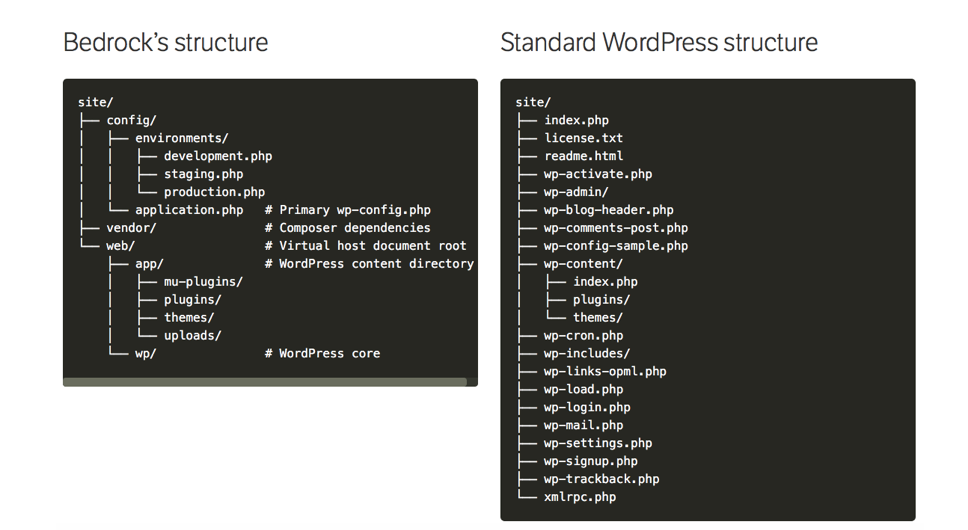
\includegraphics[trim = 0 0 0 0, clip, width=0.85\textwidth]{ph20.png}
      \caption{Difference between Bedrock and standard Wordpress Structure}
\label{bedrockfolder}
 \end{table}

Composer, a tool for dependency management in PHP, is used to pull in
both *.dotenv and WordPress, along with WordPress plugins \cite{p7}.
Suppose a developer has a project that depends on some libraries and
some of those libraries depend on other libraries. In essence, Composer
allows the developer to declare the libraries they depend on and finds
out the correct versions of packages needed and installs them into the
project \cite{p8}.

\hypertarget{trellis}{%
\subsubsection{Trellis}\label{trellis}}

Trellis is a Wordpress development and production server tool which
creates and manages these machines. Trellis makes use of Ansible, using
this software for automation of cloud provisioning, configuration
management, application deployment, and many other IT needs \cite{p12}.
These are automated across both local and production servers. To create
a local environment, a machine must be provisioned on top of a
virtualiser, such as VMWare or VirtualBox. Vagrant is then used to
implement these development environments. It is a virtual environment
manager with a focus on automation \cite{p10}. Vagrant provides work
environments that are easy to configure, reproducible, and transportable
controlled by a single reliable workflow. Then, industry-standard
provisioning tools such as shell scripts, Chef, or Puppet, can
automatically install and configure software on the virtual machine
\cite{p10}.

The combination of the Bedrock structure and Ansible automation means
that Trellis allows WordPress developers to create and manage more
professional server environments almost automatically.

\hypertarget{sage}{%
\subsubsection{Sage}\label{sage}}

Sage (sitting on top of the Trellis, Bedrock stack), provides modern
front-end development workflow designed with the idea of creating:

\begin{itemize}
\tightlist
\item
  An advanced workflow
\item
  Minimal HTML5 templates
\item
  Theme wrappers
\item
  Handy tools such as browser sync to automatically compile and check
  code across a range of device synchronously
\end{itemize}

\hypertarget{front-end}{%
\subsection{Front-End}\label{front-end}}

As the name would suggest, front-end development encompasses the
creation of the parts of a website with which the user interacts,
through the use of technologies such as HTML, CSS, and JavaScript. In
other words, this is where the site's content, styling and dynamic
interface is coded.

HyperText Markup Language (HTML), is the backbone of every website. This
is where a site's content is kept. It is in the HTML documents where a
developer uses embedded PHP to connect the site to the content
management system.

Cascading style sheets (CSS) are where a sites unique style is
developed. SCSS is a version of CSS written for SASS, a program written
in Ruby that assembles CSS style sheets for a browser. The advantage of
using SASS is that is has added functionality, allowing the use of
variables, nested rules, mixins and more within CSS-compatible syntax
\cite{p14}.

Resposive design is critical for modern websites since they are accessed
from a variety of browsers and screen sizes. To achieve a consistent,
responsive interface, Bootstrap 4, a front-end web framework based on
CSS styling, can be used. It has set of fixed classes that allow
developers to quickly create applications that scale to a variety of
device sizes. Additionally, Bootstrap aids developers in adding
conventional components such as navigation bars and panels to a site. It
has become the industry standard for responsive web development
\cite{p15}.

To add dynamic functionality to a website JavaScript (JS) is used. JS is
a front-end development language employed by many websites and supported
by all modern web browsers. JQuery is a JavaScript library that
simplifies animation, event handling and much more. It is also used to
add functionality to a website \cite{p16}.

\begin{table}[H]
      \centering
      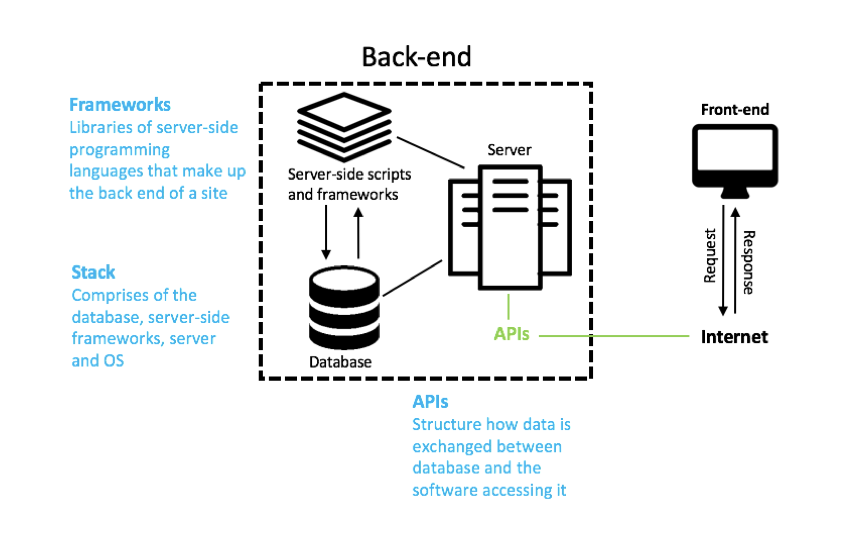
\includegraphics[trim = 0 0 0 0, clip, width=0.8\textwidth]{ph18.png}
      \caption{Front-End and Back-End Interaction}
 \end{table}

\hypertarget{back-end}{%
\subsection{Back-End}\label{back-end}}

Backend development refers to the server-side code written to ensure
that a site is robust and usable. This is the code that is run on the
server and is responsible for things such as database interactions,
logic, and calculations. PHP is a server-side scripting language used to
query a database such as MariaDB or MySQL \cite{p17}. MariaDB is a fork
of MySQL and as such has the same database structure and indexes.
\cite{p24}

If WordPress is used as the content management system, it is also
deployed on the server so that content can be updated via the
user-friendly dashboard. This then updates the database, and
strategically placed PHP embedded in HTML can be used to display the
content in the appropriate part of the site.

Blade by Laravel was is a templating engine used in conjunction with
PHP, after appending the file extension \emph{blade.php}. Blade employs
the concepts of template inheritance and sections. The \emph{@section}
notation allows for easy organisation of a site and can be embedded
inside HTML code. The \emph{@extends} notation can be used to inherit
other layouts. These tools are extremely convenient for effectively
organising code \cite{p18} meeting some of the design patterns further
discussed in Section \ref{design-patterns}.

\begin{table}[H]
      \centering
      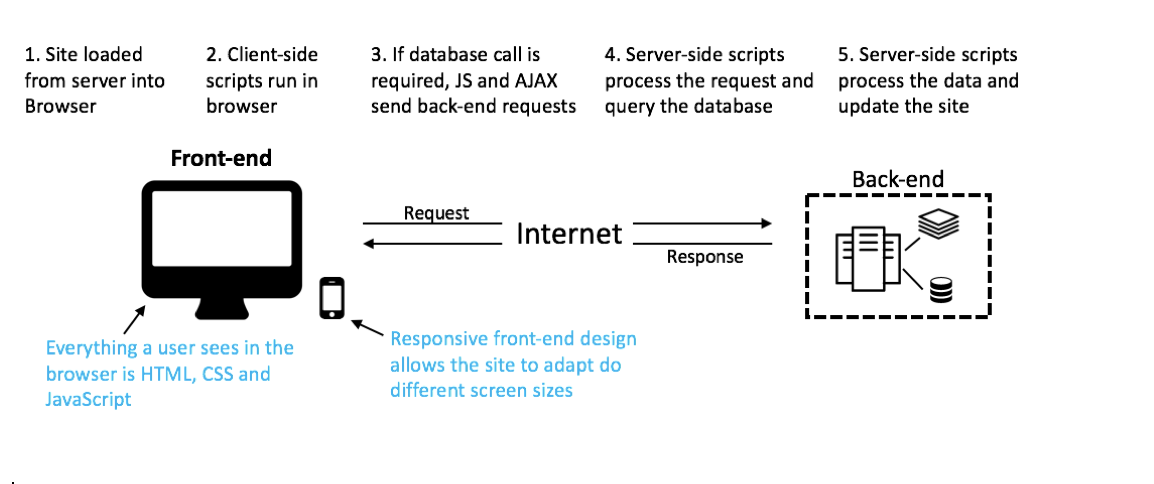
\includegraphics[trim = 0 0 0 0, clip, width=0.98\textwidth]{ph17.png}
      \caption{Front-End and Back-End interaction}
 \end{table}

\newpage

\hypertarget{system-architecture}{%
\section{System Architecture}\label{system-architecture}}

In order to be able to create a high performance website, using the
latest technologies to optimises run-time and speed up the design
process; a stack of Wordpress technologies were used in three-tier
system architecture. The stack was run across both local and production
servers enabling a testing environment which was fully representative of
the production server while all code could be kept offline.

The full open source Roots stack \cite{rootsweb} was selected as it
provided all the tools and structure required to develop the project to
a professional standard. Figure \ref{systemarchitecture} shows the
relationship between the three roots technologies; Sage, Bedrock and
Trellis, and their relationship to the system architecture.

\begin{table}[H]
\centering
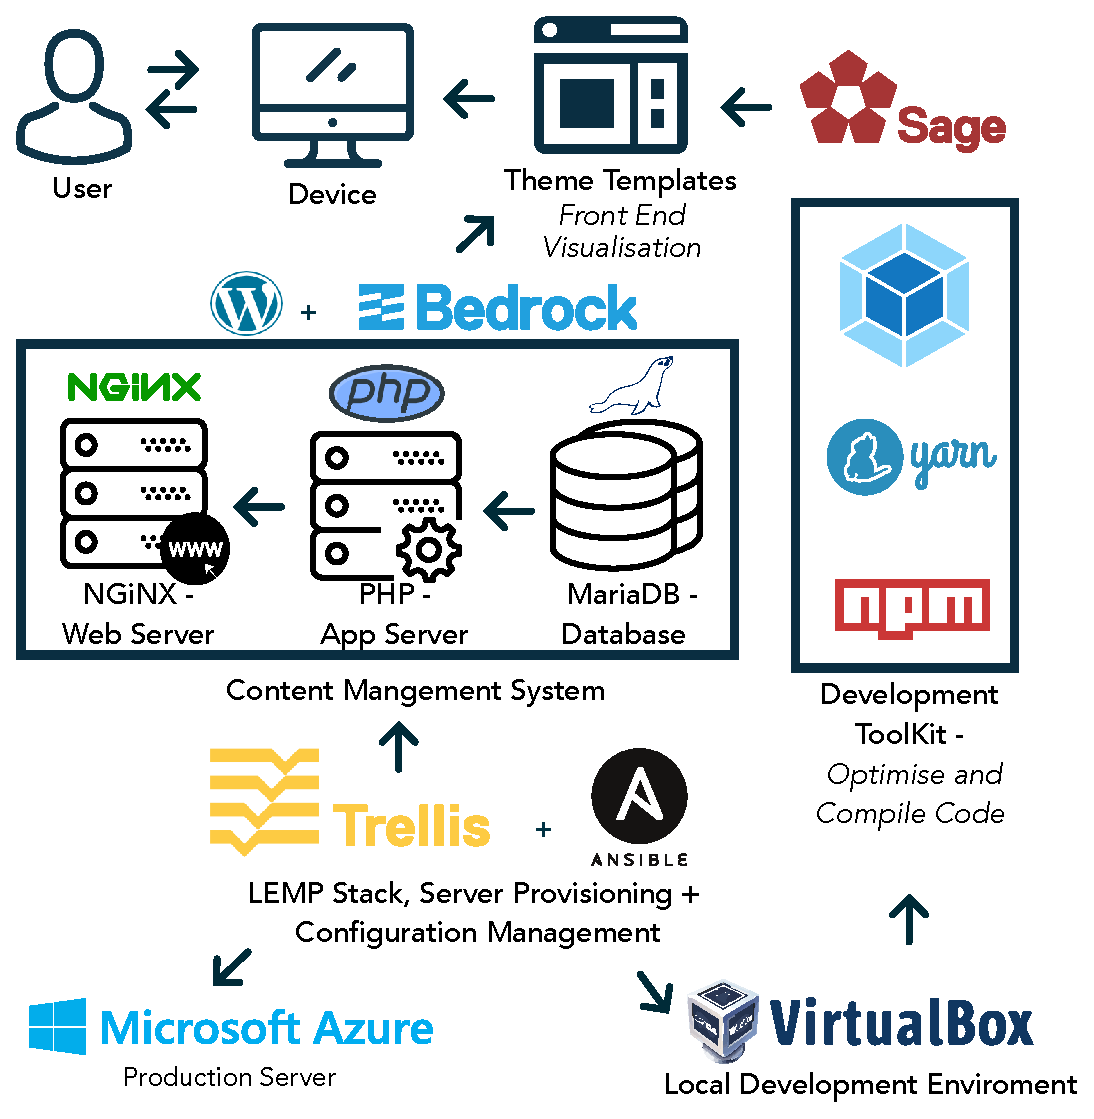
\includegraphics[trim = 0 0 0 0, clip, width=0.85\textwidth]{SystemArchitecture.eps}
\caption{Diagram showing the websites systems architecture, highlighting the relationship between different technologies}
\label{systemarchitecture}
\end{table}

\hypertarget{design-patterns}{%
\subsection{Design Patterns}\label{design-patterns}}

Due to the complexity of the IXN website's system architecture, multiple
design patterns were used; simplifying development workflow and
improving code readability. The Roots Sage starter theme was selected
because it offers many design pattern benefits off the shelf. Some of
the typical benefits of using design patterns include:

\begin{itemize}
\tightlist
\item
  The ability to reuse large amounts of code \cite{deanDesignPatterns}
\item
  Capture expert knowledge from other developers where design trade-offs
  have already been evaluated
\item
  Improve communication between the IXN development team
\end{itemize}

\textbf{Strategy:} This is where a family of algorithms are defined and
are made interchangeable depending on the client use case
\cite{gamma1995design}. This design pattern was used in the handling of
JavaScript files, splitting the files into common, main and custom.
Different JavaScript files would be loaded dependent on which page was
being called.

\textbf{Singleton:} This is where a class is ensured not to have any
more than one instance \cite{gamma1995design}. When creating PHP
functionality for the website such as Reading Time
(\texttt{reading\_time()}), found on news posts or the string chopper
tool (\texttt{chop\_string()}) these classes where defied once in the
\texttt{extras.php} file and then called using namespaces. This ensured
the classes were only created once and the functionality could be
accessed elsewhere in the code (see Figure \ref{ddcode}).

\textbf{Template Method:} This is where a skeleton is used to define
reusable components for subclasses \cite{gamma1995design}. This means
that subclasses can redefine certain steps of the over-arching class
without changing the code's structure. Through using the Larval
templating engine, a skeleton for each view could be defined in the
\texttt{app.blade.php}, different templates files could then be selected
and swapped out depending on the page selected.

\begin{table}[H]
\centering
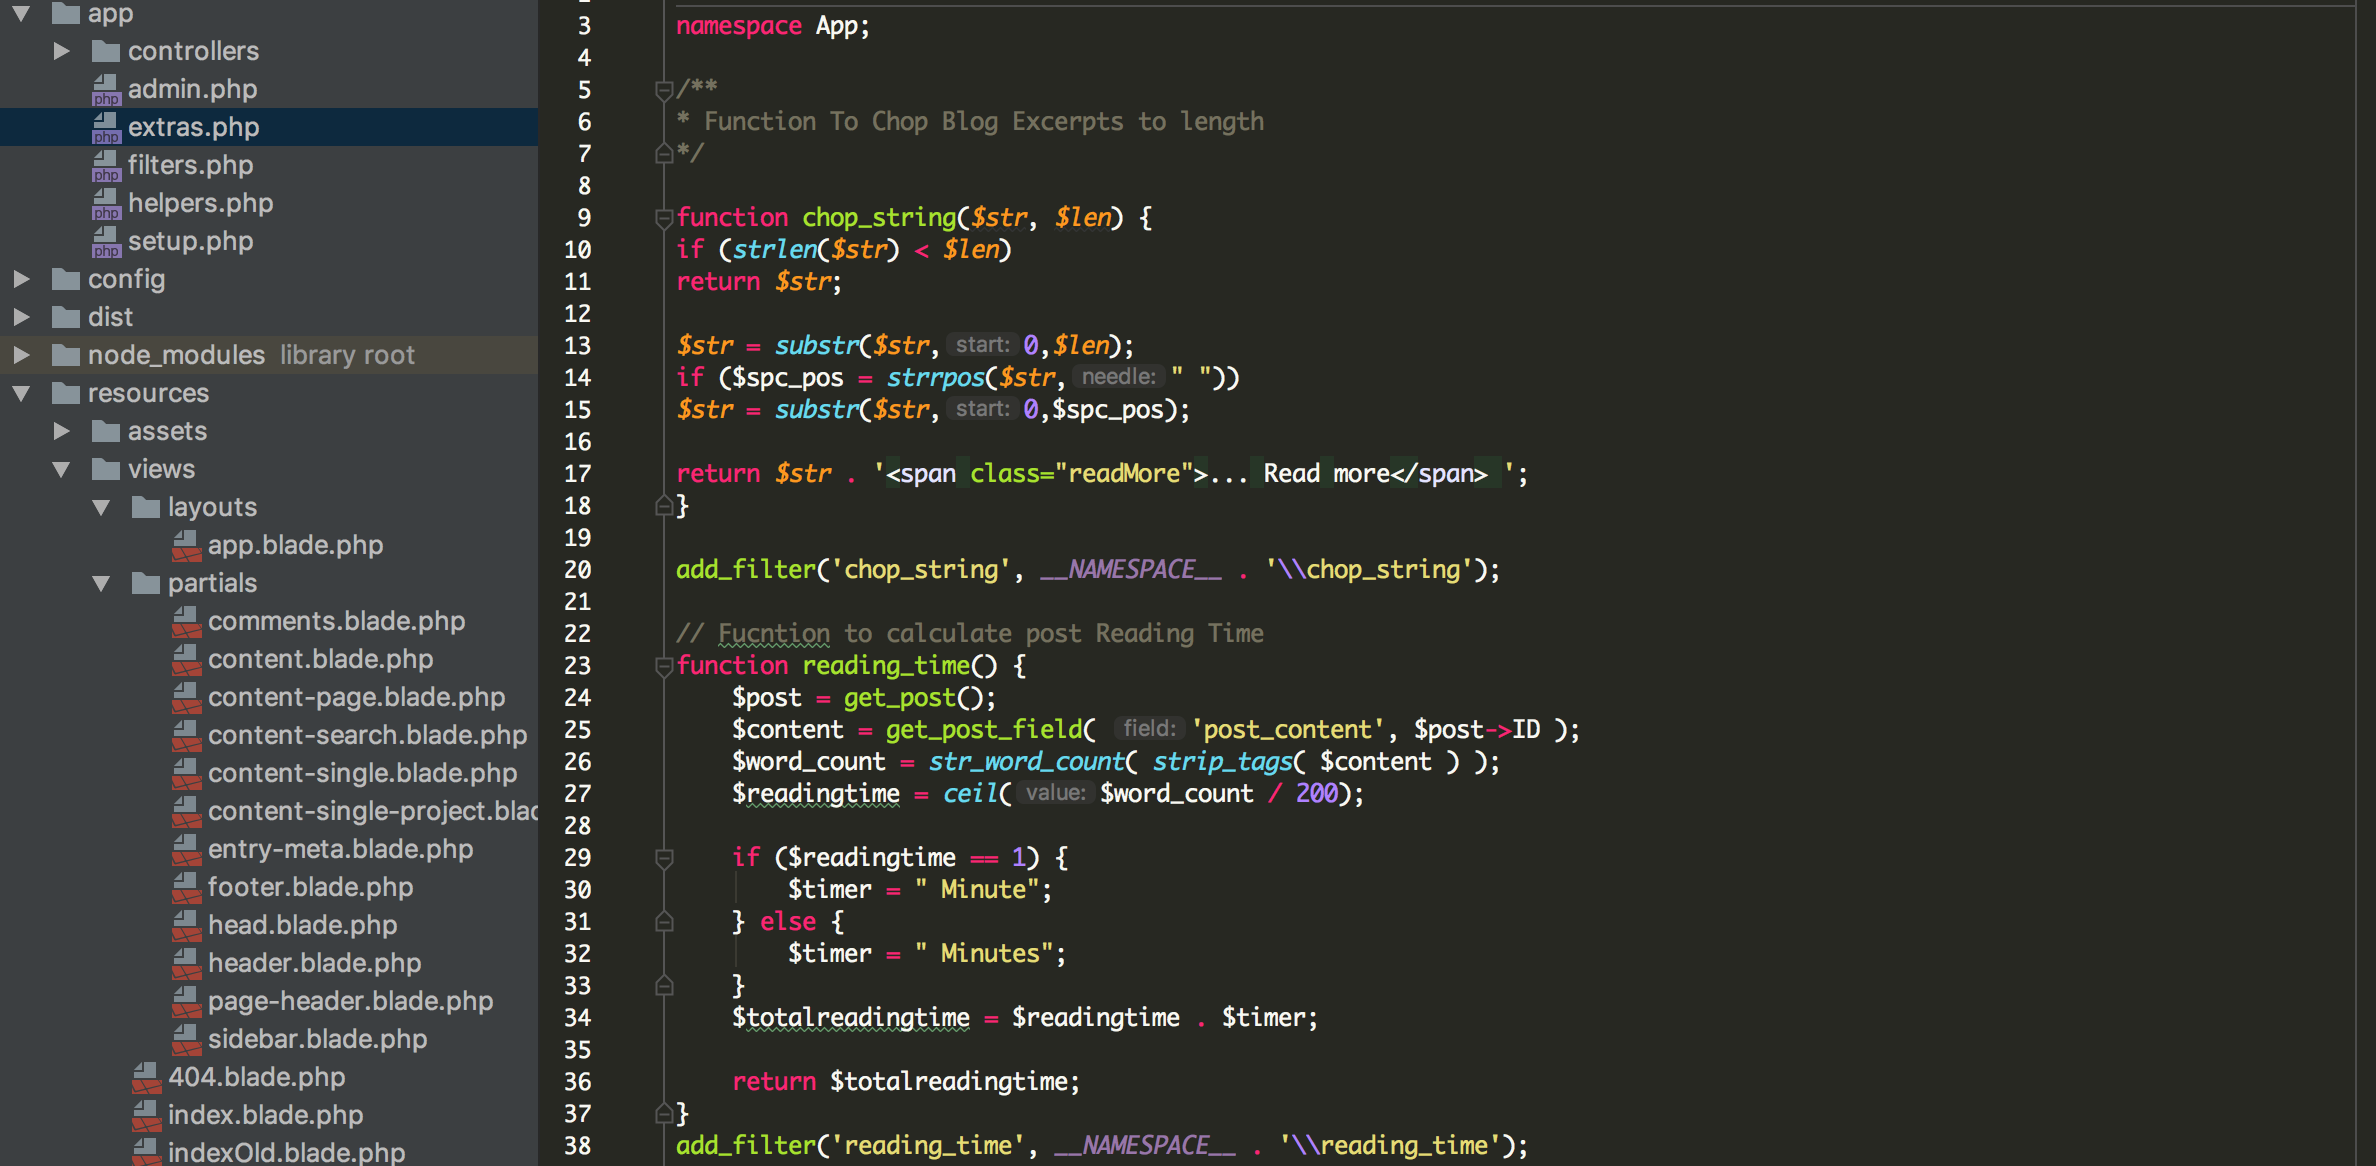
\includegraphics[trim = 0 0 0 0, clip, width=0.75\textwidth]{ddcode.png}
\caption{Overview of project code structure, including singleton design pattern in extras.php}
\label{ddcode}
\end{table}

\newpage

\hypertarget{implementation}{%
\section{Implementation}\label{implementation}}

After down researching and down-selecting the most appropriate
technologies to meet the project requirement goals, a development
environment was created and shared amongst all the members of the team.
The local development environment was then used to codify the detailed
design template (formed at the end of the design phase) into the final
product. This section discusses, the methodology and workflow of the
build cycle and deployment stages within the development phase of the
project.

\hypertarget{local-development}{%
\subsection{Local Development}\label{local-development}}

Due to the advantages discussed in Section
\ref{roots-technology-stack-sage-bedrock-and-trellis}, Trellis was used
to set up a local Ubuntu server on a virtual machine. The virtual
machine provided a sandbox to test and develop the IXN website
replicating the characteristics of a live production server. After
installing Trellis's dependencies on a developers computer, and
configuring specific files; Trellis can be run to create a local
development environment automatically; building a local server on a
virtual machine, provisions all full LEMP stack and Wordpress
installation \cite{p21}.

\hypertarget{file-configuration}{%
\subsubsection{File Configuration}\label{file-configuration}}

Configuring of the Trellis requires few simple steps. Within the Trellis
file directory a collection of files were edited including:

\begin{itemize}
\tightlist
\item
  \texttt{group\_vars/development/wordpress\_sites.yml}
\item
  \texttt{group\_vars/development/vault.yml}
\end{itemize}

These files configure the server name and allow for multisite
installation to be created. Using Ansible's inbuilt encryption software,
all \texttt{.vault} files were encrypted; preventing any passwords to be
read when committing the code to github.com. Files setup only required
completing once, shared across GitHub to other team members.

\hypertarget{server-provisioning}{%
\subsubsection{Server Provisioning}\label{server-provisioning}}

Finally, typing \texttt{vagrant\ up} and \texttt{vagrant\ provision} in
the command line while within the Trellis directory would run the
Trellis software. Vagrant and Ansible complete most of the heavy
lifting, two Trellis dependency packages, which uses a Vagrantfile and a
collection of Ansible \texttt{*.yml} files to set up a virtual machine
\cite{p22}. By using the Trellis setup, a similar workflow can be used
to provision and deploy to a production server.

\hypertarget{development-tools}{%
\subsection{Development Tools}\label{development-tools}}

On completing the design phase discussed in Section
\ref{user-interface-design}, the design template could be split up into
components that could be individually codified by each team member, and
then brought together into the final Wordpress theme. Through combining
Bedrock with the Sage starter theme with a collection of development
tools, an efficient workspace and workflow were used.

\hypertarget{text-editors-intergrated-development-environmets-ides}{%
\subsubsection{Text Editors / Intergrated Development Environmets
(IDEs)}\label{text-editors-intergrated-development-environmets-ides}}

\begin{itemize}
\tightlist
\item
  \emph{CodePen:} Used to make each component for the website before all
  of the sections were integrated into the appropriate page layouts. The
  benefit of using CodePen is that HTML, CSS and JavaScript code can be
  written in the browser, and compiled in real time, with the result
  visible in the same window. \cite{p19} Ultimately, it allows for
  faster development and easy troubleshooting focusing on design
  problems alone
\item
  \emph{Atom/ Sublime}: These are lightweight text editors that utilise
  plugins to give additional functionality. These tools useful for
  tweaking the site and writing HTML code
\item
  \emph{PHP Storm:}, An advanced IDE, used predominantly for writing PHP
  and optimising SCSS code.
\end{itemize}

\hypertarget{collaboration}{%
\subsubsection{Collaboration}\label{collaboration}}

GitHub was used as the version control system for creating the IXN
website. Github allows revisions in the code to be stored neatly and
chronologically. The changes can then be seen by other developers who
can download and modify it using tools such as Github Desktop.
\cite{p20} GitHub is the community of developers and where they store
their work. For the IXN website there was a group repository where code
was shared and updated. To organise project code and ensure the
integrity of the site, five branches were made; two master branches and
a branch for each developer (Alexcode, PhoebeCode and GioCode). When
updates were finalised, code from the developer branches was merged into
the Dev branch. This code was reviewed, and if there were no clashes,
the code could then be to the master branch. The master housed the
cleanest and most current version of the site at any given time and was
used. The master branch was used as the code base for deployment
ensuring only stable code would be deployed. Figure \ref{githubcollab}
highlights the branch structured used in code collaboration.

\begin{table}[H]
    \centering
    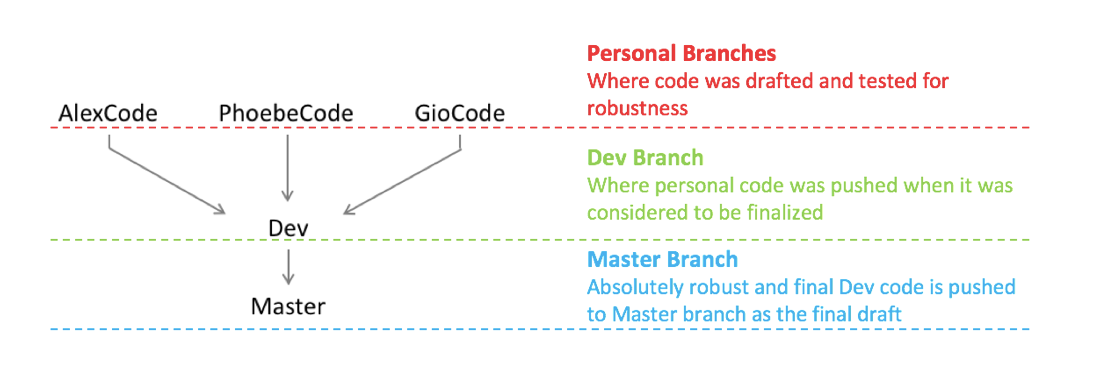
\includegraphics[trim = 0 0 0 0, clip, width=0.98\textwidth]{ph15.png}
    \caption{Overview of Github Collaboration Workflow}
  \label{githubcollab}
\end{table}

\hypertarget{web-technologies}{%
\subsubsection{Web Technologies}\label{web-technologies}}

The following technologies were used to create the front end interface
of the IXN website. After using the Trellis development environment, the
team could fully focus on creating a Wordpress theme. A theme acts like
a skin which sits on top of the Wordpress CMS, providing the look and
feel users interact with. Through using the Sage starter template, the
following list of web technologies could be used out of the box.

\begin{itemize}
\tightlist
\item
  \emph{HTML:} used for organising webpage structure
\item
  \emph{Bootstrap 4:} enhancing HTML code through providing easy to use
  classes making the website responsive. Bootstrap 4 offers many
  advantages over Bootstrap 3 including an enhanced grid system and SCSS
  as standard \cite{Differen19:online}
\item
  \emph{SCSS:} a pre-processor styling language providing additional
  functionality to basic CSS and allowing the styling sheet to be
  compiled, optimised and minified into a single CSS file named
  \texttt{main.css}. SCSS was organised into three main folders holding
  the components, layouts and global styles. This framework greatly
  improved the readability of the code and SCSS \emph{variables}and
  \emph{mixins} could then be used throughout the files to enable quick
  revision throughout the entire code base
\item
  \emph{JavaScript + (JQuery):} used to make pages interactive adding
  client-side programming functionality to the site. Javascript was used
  to make the nav-bars interactive, add video and map support among
  other features
\item
  \emph{PHP 7.1:} used as the server side language to interact with the
  server pulling out the correct content to display such as news and
  event post content.
\item
  \emph{Larvavel (Blade): } This is the templating engine used to avoid
  code repetition in keeping with the design patterns discussed in
  Section \ref{design-patterns}
\item
  \emph{AJAX:} used to allow the website to send and retrieve data from
  a PHP server asynchronously without refreshing the page. This
  technology was key to create an effective project post sorter
\item
  \emph{Shell Scripting: } small shell scripts were written to automate
  database and upload syncing between different server environments
\end{itemize}

\hypertarget{build-cycle}{%
\subsection{Build Cycle}\label{build-cycle}}

To implement the IXN website efficiently, a build cycle highlighted in
Figure \ref{designprocess} was followed to allow for an agile
development process. Each team member was assigned single components to
design, construct and test. This decision was made to streamline and
facilitate the process making the webpage testing and tweaking
components for different screen sizes and browsers until the element was
ready to integrate into the final code base. The build process can be
summarised in the following steps:

\begin{enumerate}

\tightlist
\item
  Using the Sketch detailed design template, the component CSS could be
  exported giving the rough parameters for font shape and size
\item
  CSS code was placed into CodePen where HTML and JS were used to
  construct the component in full-screen size. This tool was chosen due
  to its' ability to display new changes in the HTML and CSS instantly
  without the need of any local development setup.
\item
  Bootstrap 4 code would then be added to, and the code base would be
  tweaked to make the component fully responsive working in every screen
  size
\item
  Code created on Codepen was then transferred to a text editor and
  integrated into the development site. This was statically tested in
  the local environment, fixing any integration problems that may have
  occurred
\item
  Once the local environment displayed positive static results, PHP was
  embedded in the HTML code to enable and simplify the connection to
  WordPress and the Maria DB database.
\item
  Another element was chosen, and the iterative process was followed all
  over again.
\item
  On completion of all components, the integrated site would be tested
  across a range of browsers, and any fixes would then be made
\end{enumerate}

Through following the build cycle, a minimum viable product (MVP) could
be quickly created allowing progress to be shown to the client and
enhancements to be made with ease. Figure \ref{buildcycleimg} shows an
overview of the different steps of the build cycle.

\begin{table}[H]
      \centering
      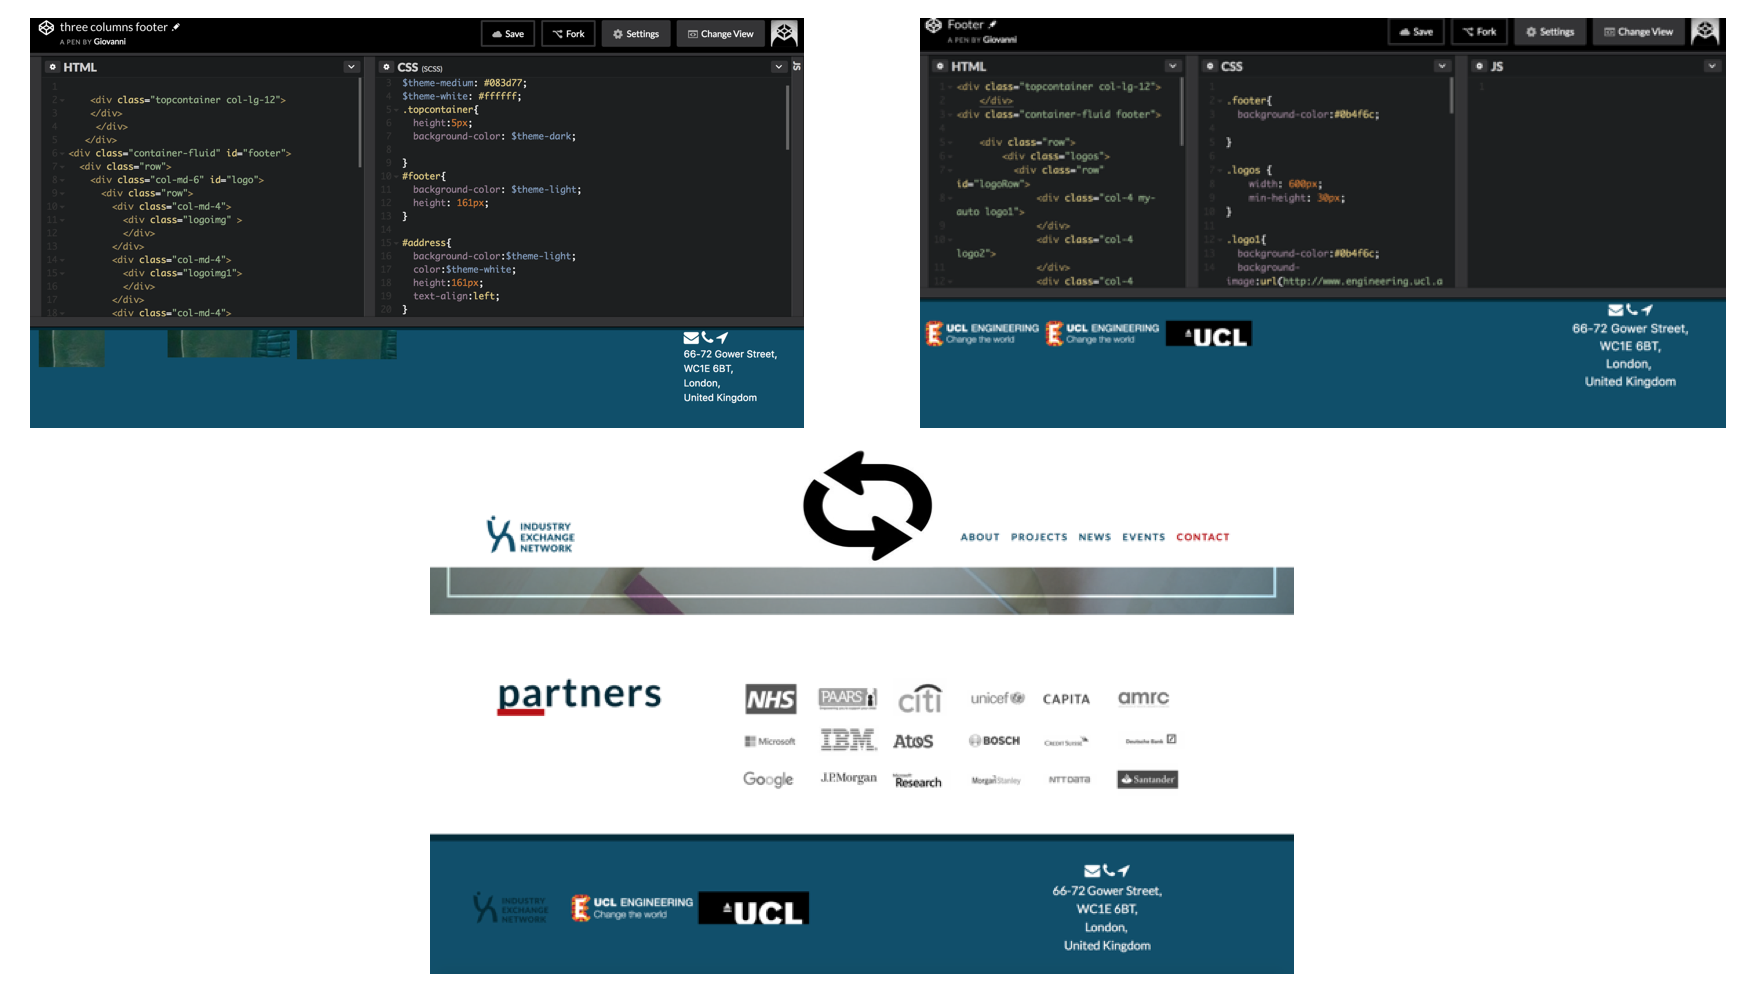
\includegraphics[trim = 0 0 0 0, clip, width=0.98\textwidth]{ph21.png}
      \caption{Iteration process followed to create the footer of the IXN website}
\label{buildcycleimg}
 \end{table}

\hypertarget{deployment}{%
\subsection{Deployment}\label{deployment}}

On completion of the build cycle, the code base was ready to be deployed
to a live production server. Due to the client's relationship with
Microsoft, Azure was selected as the production server to use providing
more than enough performance to run the IXN website.

\hypertarget{azure-setup}{%
\subsubsection{Azure Setup}\label{azure-setup}}

Using the Azure dashboard, a new blank Ubuntu 16.0.4 server was deployed
on a paid service plan which met the websites performance requirements.
The lead developers SSH key added enabling easy access to connect to the
remote server. The domain name \texttt{ixn.host} was purchased via
Namecheap selected due to its low cost. This was directed to the
production server using A name records. Finally, to allow inbound
connections to the server, port 80 required being changed to open.

\hypertarget{remote-server-connection}{%
\subsubsection{Remote Server
Connection}\label{remote-server-connection}}

To deploy to the remote server via the local development environment, a
couple of extra steps were needed the production server required Trellis
to connect, Provision and Deploy. Provisioning was done to ensure
MariaDB, Wordpress and Nginx were installed. Nginx was configured, and a
database was set up for the IXN site. The server was provisioned using
server.yml. The deployment was done using deploy.yml which compiles the
codebase from the master branch on GitHub created config files and
reloaded Nginx. \cite{p23}.

Code can be deployed after writing the following lines on the command
line in the Trellis directory:

\begin{itemize}
\tightlist
\item
  \texttt{ansible-playbook\ server.yml\ -e\ env=production}
\item
  \texttt{./bin/deploy.sh\ production\ ixn.host}
\end{itemize}

\newpage

\hypertarget{testing}{%
\section{Testing}\label{testing}}

\hypertarget{compatibility-responsiveness}{%
\subsection{Compatibility \&
Responsiveness}\label{compatibility-responsiveness}}

The team researched which browser simulators to use for testing the
compatibility and responsiveness of the IXN website. BrowserStack was an
attractive option because of the range of emulators that the tool offers
\cite{g6}. BrowserStack offered the possibility of testing the IXN
website on a multitude of Operating Systems, Devices and Browsers. The
team tested the IXN project on physical devices as well. The results
obtained for desktops and laptops are displayed below:

\begin{table}[H]
      \centering
      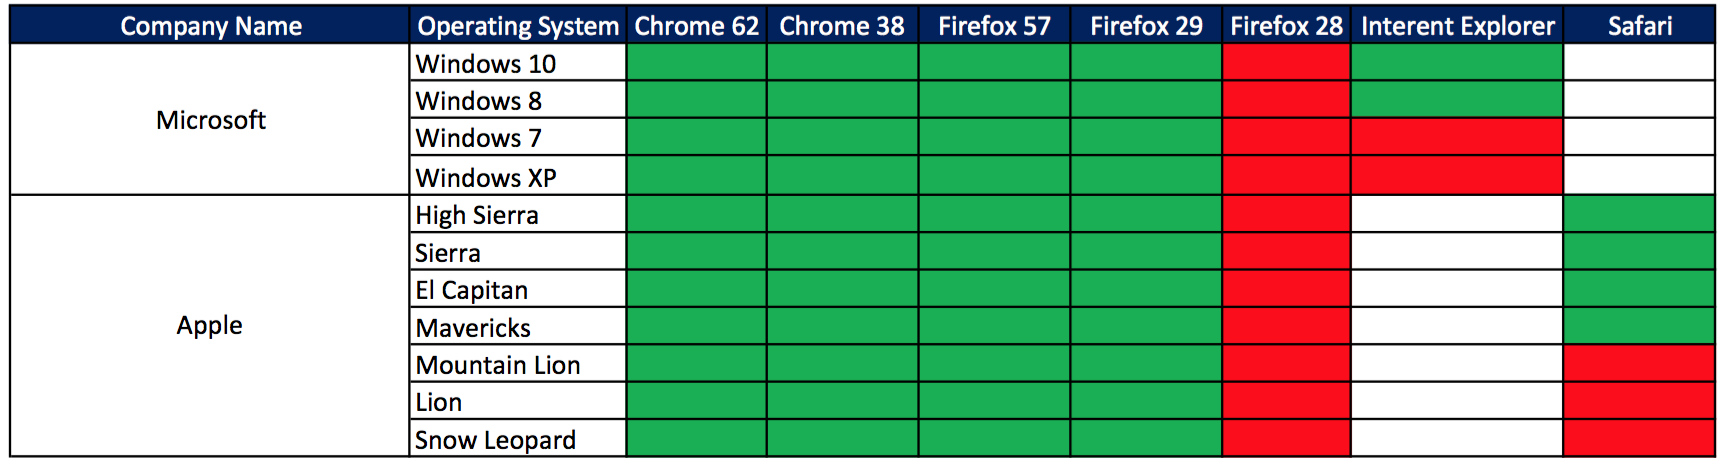
\includegraphics[trim = 0 0 0 0, clip, width=0.7\textwidth]{ph7.1.png}
      \caption{Laptop/Desktop browser testing results}
 \end{table}

In regards to testing on mobile devices, BrowserStack was the chosen
platform. However, physical device testing also played a very important
role. The webpage appears fully responsive on the most current browsers,
however, as occurred with the desktop devices older versions of software
(around 2012/2013) struggle with the design, SCSS and Bootstrap 4. The
mobile testing results are displayed below:

\begin{table}[H]
      \centering
      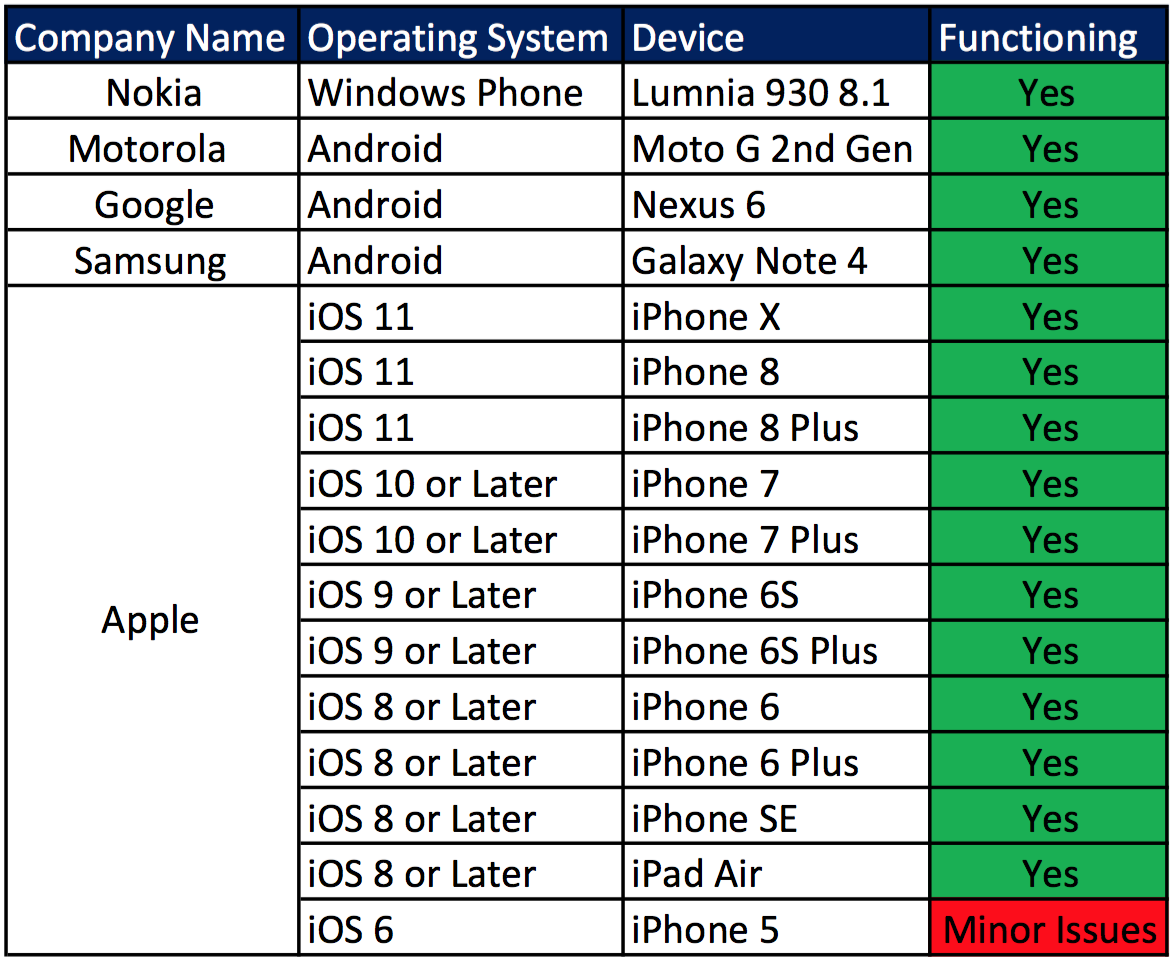
\includegraphics[trim = 0 0 0 0, clip, width=0.7\textwidth]{ph8.png}
      \caption{Mobile browser testing results}
 \end{table}

\hypertarget{server-stability-issues}{%
\subsection{Server Stability Issues}\label{server-stability-issues}}

The team has encountered issues in launching the website through
Microsoft Azure due to the complexity involved in the process of setting
up a stable server. The browsers sporadically showed that the page was
not redirecting properly or that the page was in a redirect loop. The
problem seemed to disappear after the website had been reloaded a second
time. The team, in the last days before the deadline, was able nearly
totally fix this problem resulting in a very improved server stability.
Future teams working on the IXN project will have to run more robust
tests to see to what extent the issue is still present.

\hypertarget{acceptance-testing}{%
\subsection{Acceptance Testing}\label{acceptance-testing}}

The IXN User Acceptance Testing (UAT) has been generated around the
requirements of the website \cite{g7} . Use Cases have been used to pick
and prepare tasks for users to perform during testing. The procedure
that the IXN team followed for User Acceptance Testing is the following:
1. Design tests for users to cover functional scenarios of the website
2. Select a testing team of individuals from a variety of backgrounds 3.
Perform the tests and record the results 4. Fix the bugs encountered or
improve the inadequate features.

For the IXN website UAT, thirty-five individuals of varied technical
backgrounds were asked to complete the tasks given and the time of
completion was recorded. The table below summarises the results
obtained:

\begin{table}[H]
      \centering
      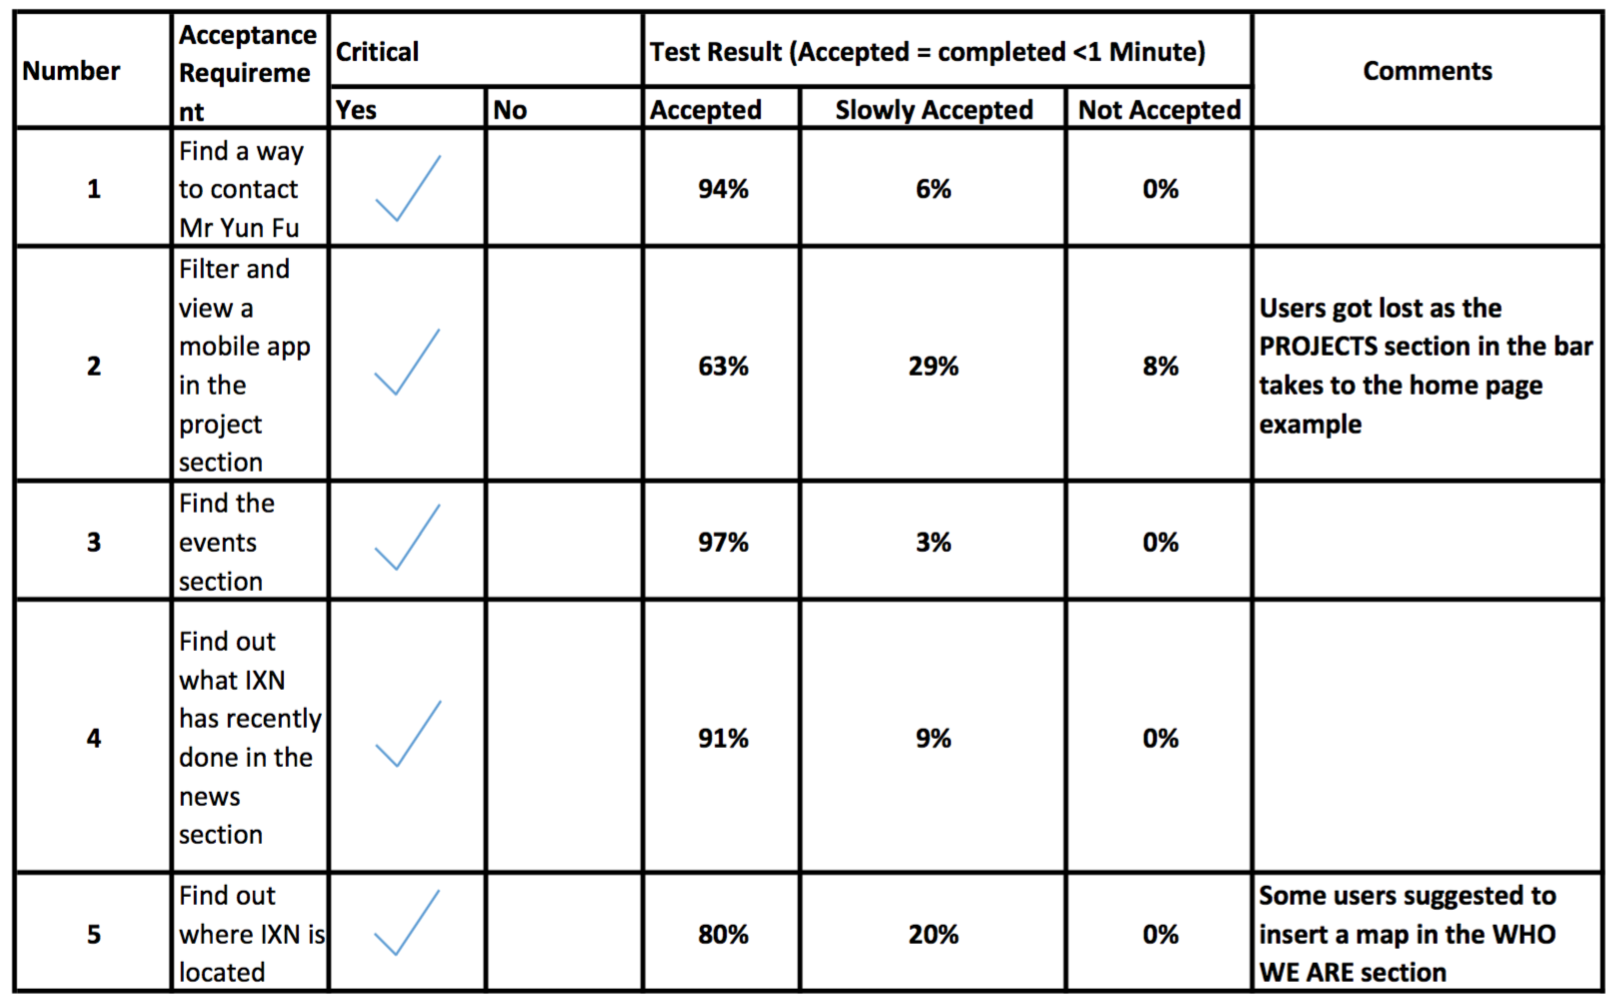
\includegraphics[trim = 0 0 0 0, clip, width=0.7\textwidth]{ph4.png}
      \caption{User Acceptance Testing summarised results}
 \end{table}

\hypertarget{error-guessing}{%
\subsection{Error Guessing}\label{error-guessing}}

Error guessing has been put into practice by making the most of the
expertise of fellow UCL Computer Science Students. The IXN team asked
members of the Department of Computer Science to come up with, consider
and assess circumstances in which the software behind the website might
have had problems in coping with the requests made. The efficiency of
this testing technique depends on the tester's abilities. In the case of
the IXN website, some minor bugs were spotted in the news section.
Consequently, the team went on to fixing them.\# Conclusion

\hypertarget{requirements-accomplishments}{%
\subsection{Requirements
Accomplishments}\label{requirements-accomplishments}}

When comparing the MoSCoW requirements to the team achievements, it is
evident that all of the ``Must-have'' (in green) and ``Should-have'' (in
yellow) requirements were fulfilled. An extra ``Could-have'' (in red)
feature was also included to give a more comprehensive user experience.
An annotated MoSCoW, explaining how the requirements were implemented,
can be found below:

\begin{table}[H]
      \centering
      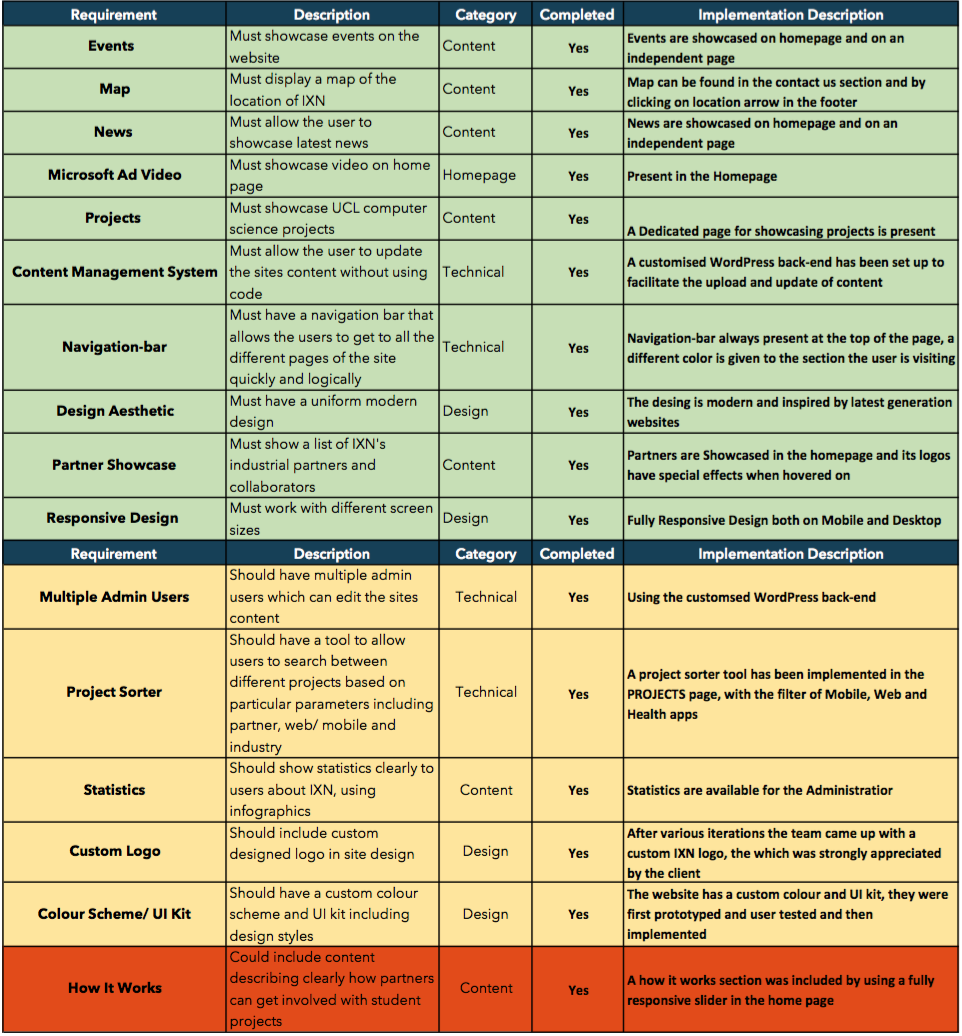
\includegraphics[trim = 0 0 0 0, clip, width=0.7\textwidth]{ph5.png}
      \caption{Post implementation annotated MoSCoW}
 \end{table}

\hypertarget{team-achievements}{%
\subsection{Team achievements}\label{team-achievements}}

Teamwork presented several advantages and disadvantages. The IXN team
faced a few challenges concerning background knowledge, workload
division and the different culture of its team members. There were times
of disagreement between team members, however, through open-minded
discussion, honesty, cooperation and respect every individual gained
valuable experience and new skills throughout the development of the
website.

While additional technical features and subtle design improvements may
have been possible with additional time, the final overall look and
functionality of the site were satisfactory given the module
constraints. Overall, the team was happy with the final result of the
IXN website.

\hypertarget{critical-evaluation-future-development}{%
\subsection{Critical Evaluation \& Future
Development}\label{critical-evaluation-future-development}}

The project was highly design-focused. Therefore, the team worked
tirelessly to make the site attractive, simple-to-use and polished.
However, site maintenance is crucial for the continued efficacy of the
site.\cite{g8} The role of future developers working on the IXN website
will, therefore, be to build upon the foundations that have already been
created. Some points of focus could be:

\begin{itemize}
\tightlist
\item
  Improving/expanding site content: Continuously updating the latest
  projects, news, and events
\item
  Improving/expanding upon the WordPress Admin Panel: Optimizing the
  panel to exact admin specifications
\item
  Simplifying the post-adding method: Make adding new project, news and
  events posts more intuitive
\item
  Improve site speeds and performance: Optimize Azure server
  configuration and site file optimization (minifying CSS, JS etc.) to
  avoid current occasional redirect errors. Use Google site speed checks
  to find weaknesses in current performance
\item
  Improved search optimisation: Use of plugins (eg: YOAST)
\item
  Improved data analytics: Connect to client's Google analytics account
\item
  Further improvements based on more thorough user-testing: Evaluate
  user response to current site through exhaustive user-based testing to
  make a more data-driven site design and functionality
\end{itemize}

Moreover, the additional and less requested requirements of the
``Could'' section of the MoSCoW can be taken consideration and
implemented. A commented version of the ``Could'' portion, explaining
how the features can be realised, is present below:

\begin{table}[H]
      \centering
      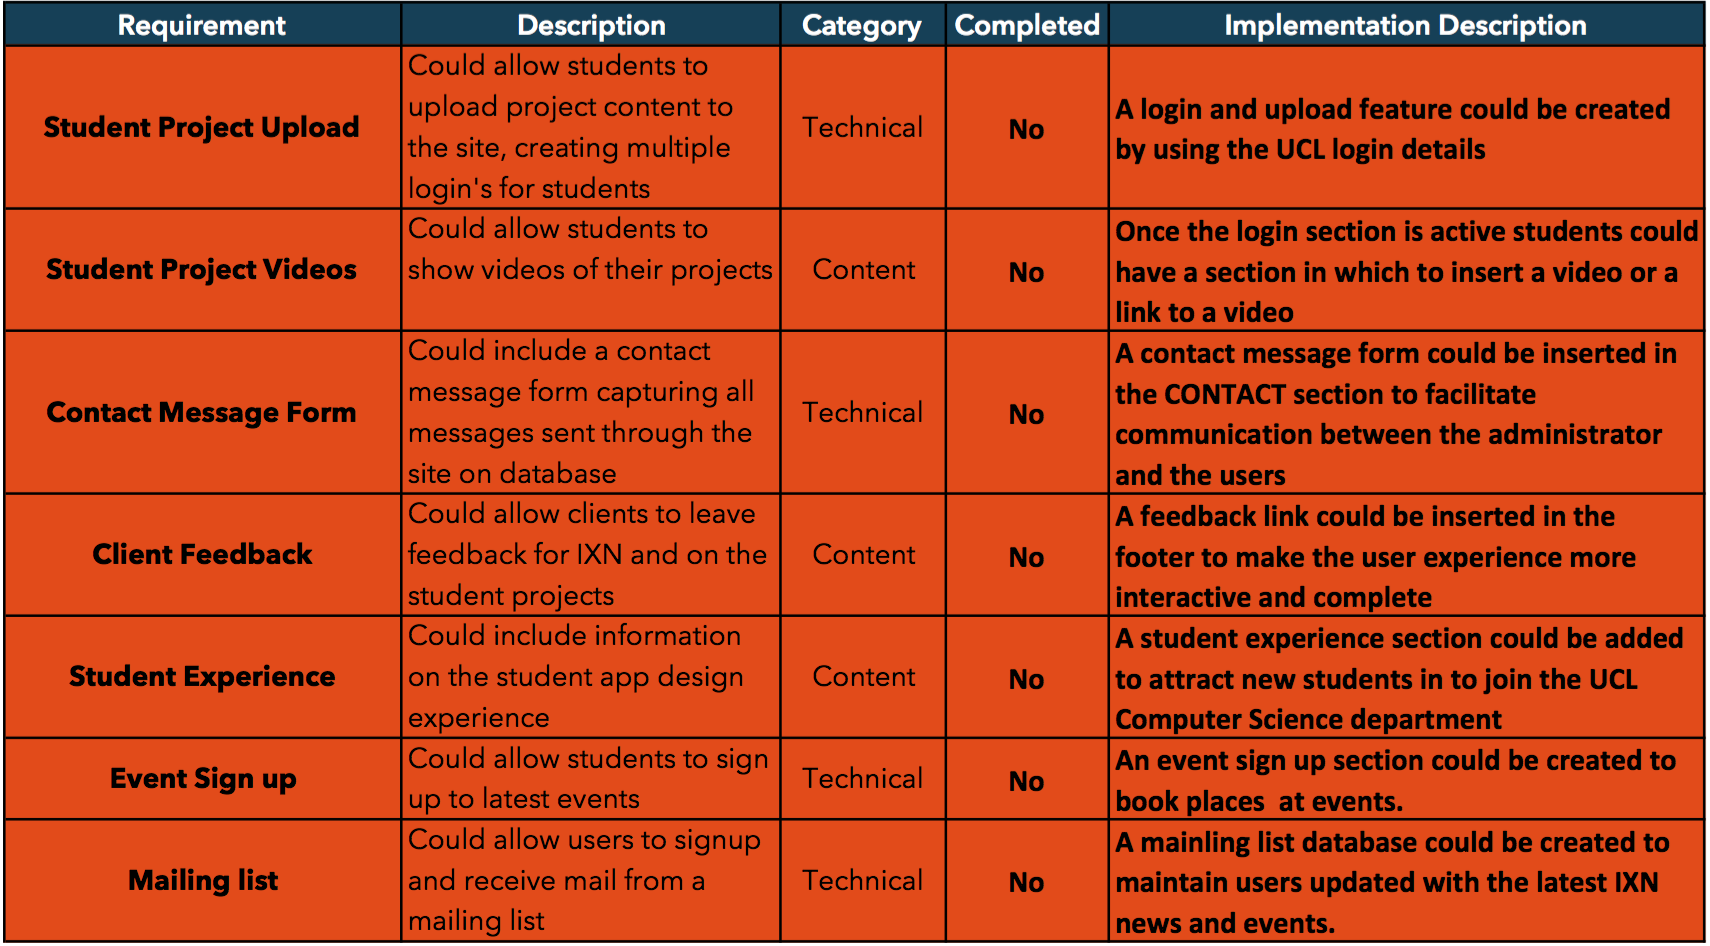
\includegraphics[trim = 0 0 0 0, clip, width=0.7\textwidth]{ph6.png}
      \caption{Possible features to be implemented in the future}
 \end{table}
% -----------------------------------------------------------------------------------
%                               BIBLIOGRAPHY - Insert Name of BIB File Here
% -----------------------------------------------------------------------------------
\newpage

% ---------------BIBTEX OLD-----------------------------------------------------
% \bibliographystyle{unsrt} %%%% Plain or alpha can change orders here
% \bibliography{BibFile}
% \nocite{*} %%%if you want to see all references even those note cited in the text
% -----------------------------------------------------------------------------------

\printbibliography
% -----------------------------------------------------------------------------------
%                                  APENDIX
% -----------------------------------------------------------------------------------

% \end{counted} %<<<<<<<<<<<<<<ENDS WORD COUNTER

\newpage
\section{Appendices}

\subsection{Login Guide}
\begin{itemize}

  \item Go to WordPress Login Page at ixn.host/wp-admin
  \item Use the Username: YunFu
  \item Use the Password: AppDesign

\end{itemize}

\begin{landscape}
\subsection{Competing Solutions}
  \begin{figure}[H]
      \centering
      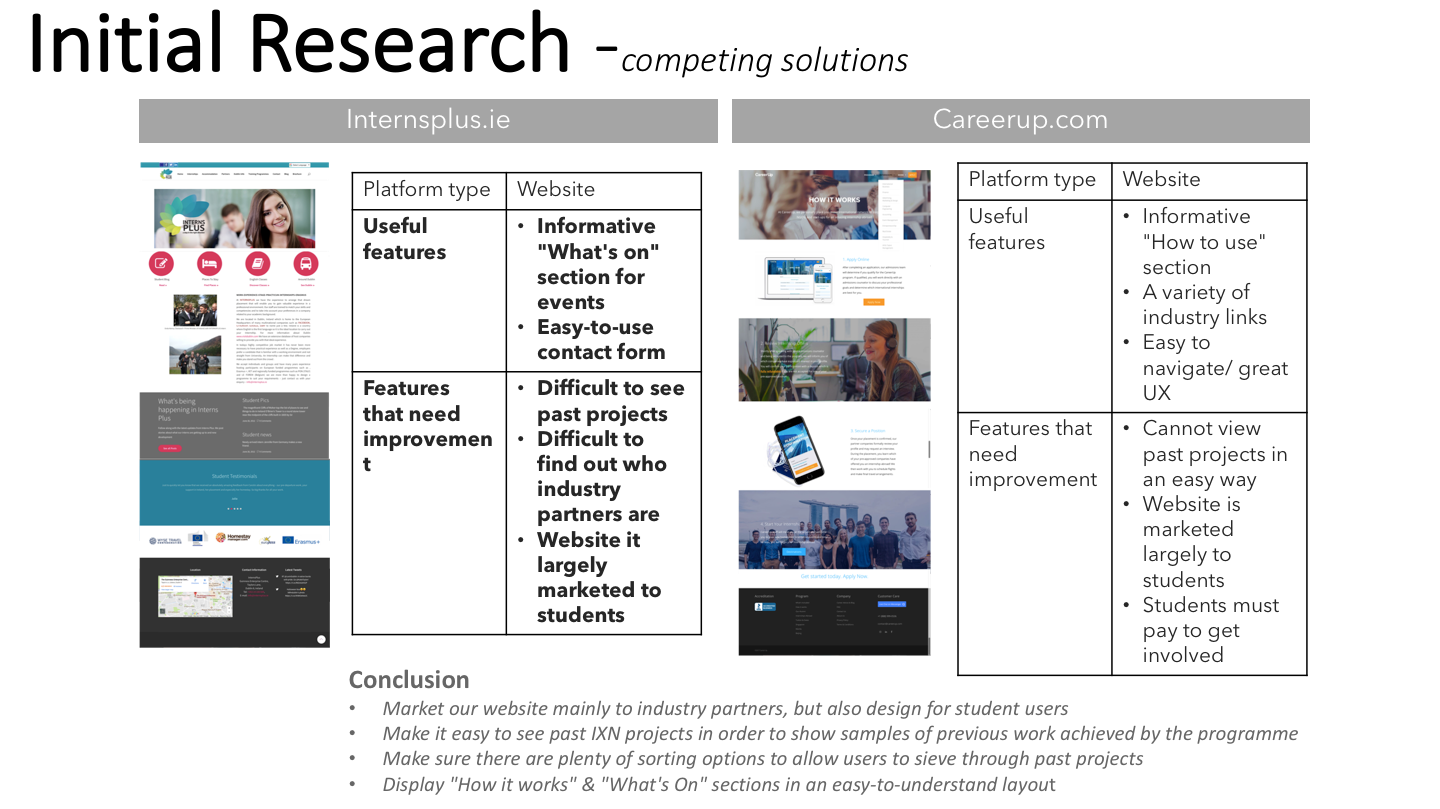
\includegraphics[trim = 0 0 0 0, clip, width=0.99\textwidth]{app5.png}
      \caption{Possible features to be implemented in the future}
 \end{figure}
 \end{landscape}

 \newpage


\begin{landscape}
\subsection{Sketches}
 \begin{figure}[H]
      \centering
      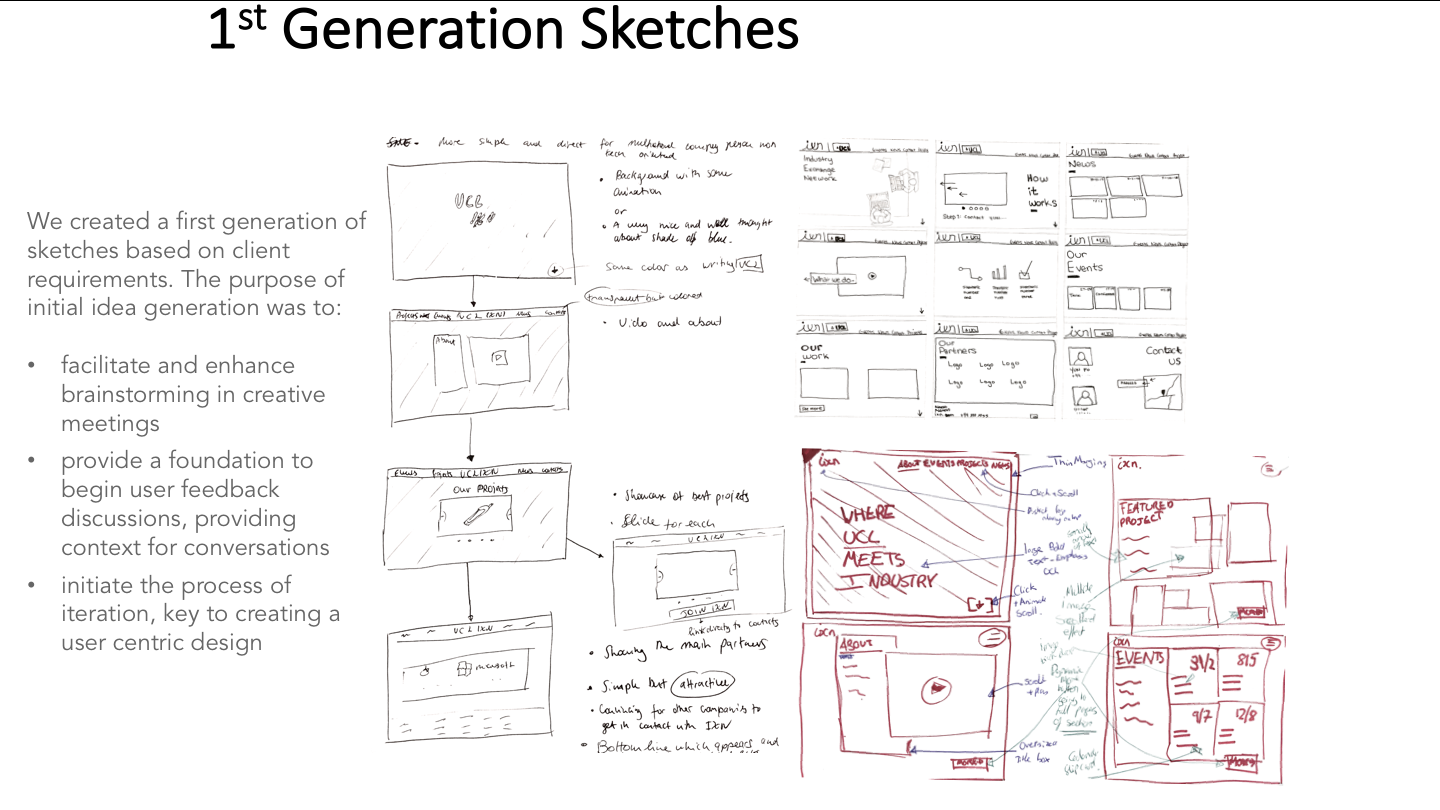
\includegraphics[trim = 0 0 0 0, clip, width=0.99\textwidth]{app4.png}
      \caption{First generation hand-drawn sketches}
 \end{figure}
\end{landscape}

 \newpage

\begin{landscape}
 \begin{figure}[H]
      \centering
      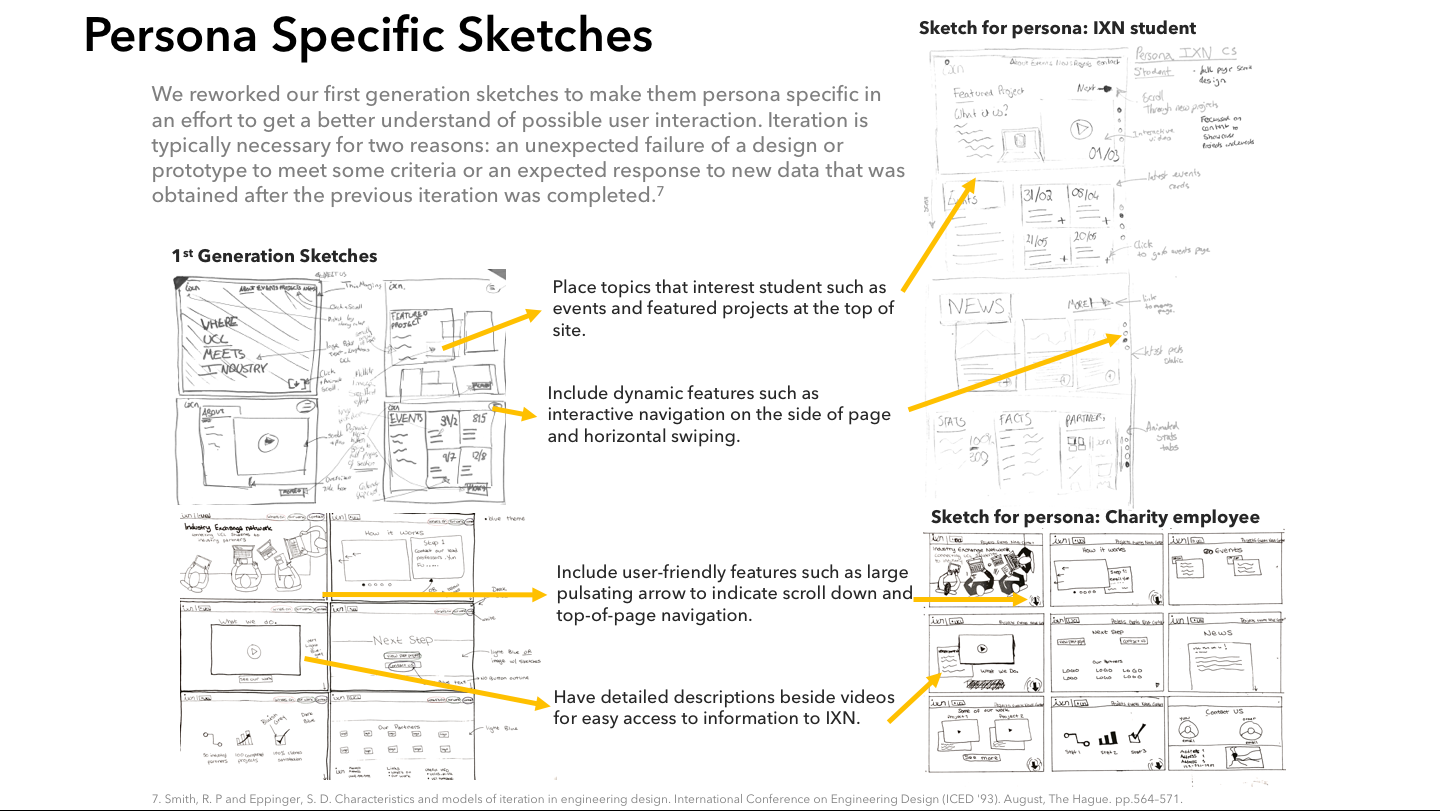
\includegraphics[trim = 0 0 0 0, clip, width=0.99\textwidth]{app3.png}
      \caption{Sketches based on researched personas}
 \end{figure}
  \end{landscape}

\newpage

\begin{landscape}
\subsection{Storyboards}
 \begin{figure}[H]
      \centering
      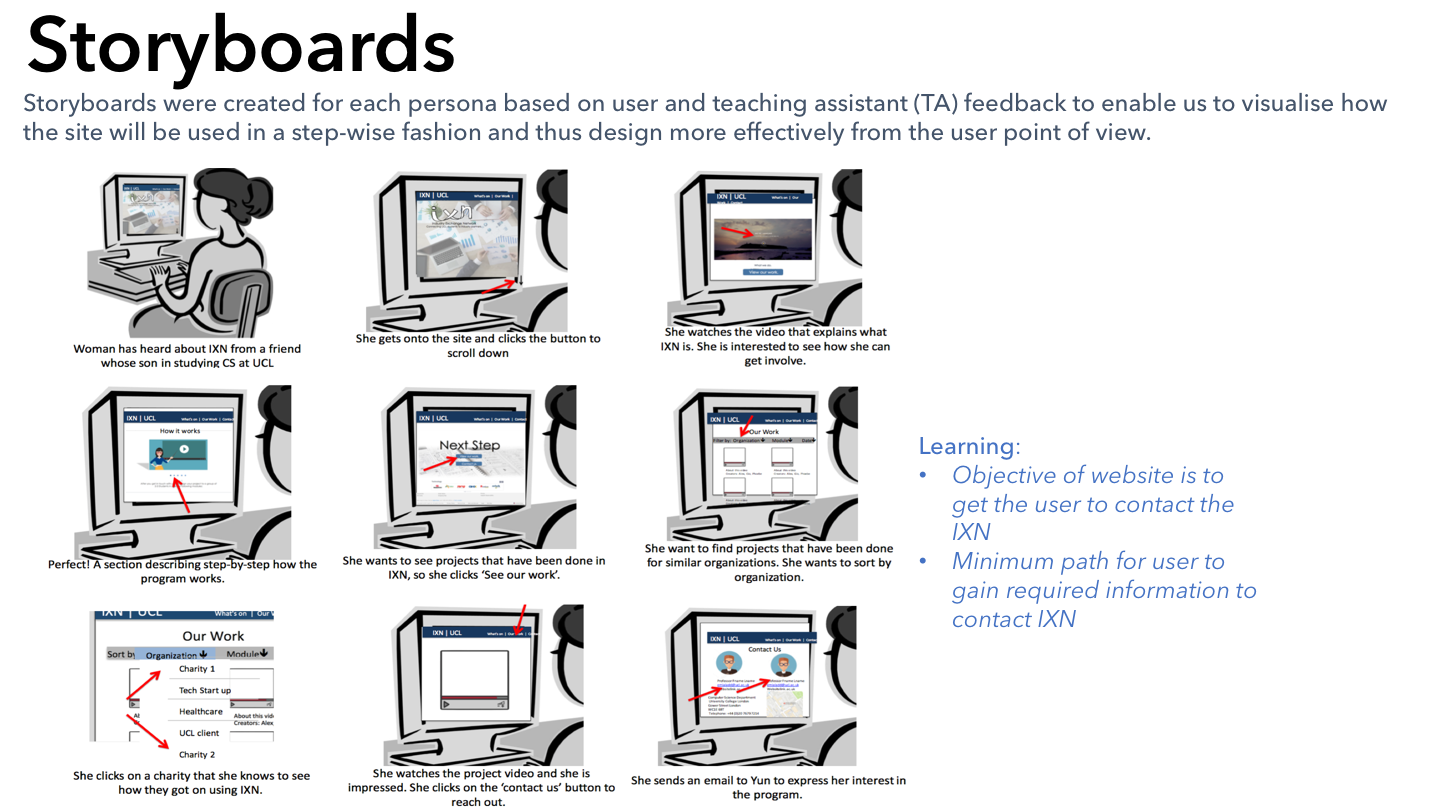
\includegraphics[trim = 0 0 0 0, clip, width=0.99\textwidth]{app2.png}
      \caption{Storyboard example describing a possible user experience.}
 \end{figure}
\end{landscape}

 \newpage

\begin{landscape}
\subsection{Wire-Framing}
\begin{figure}[H]
      \centering
      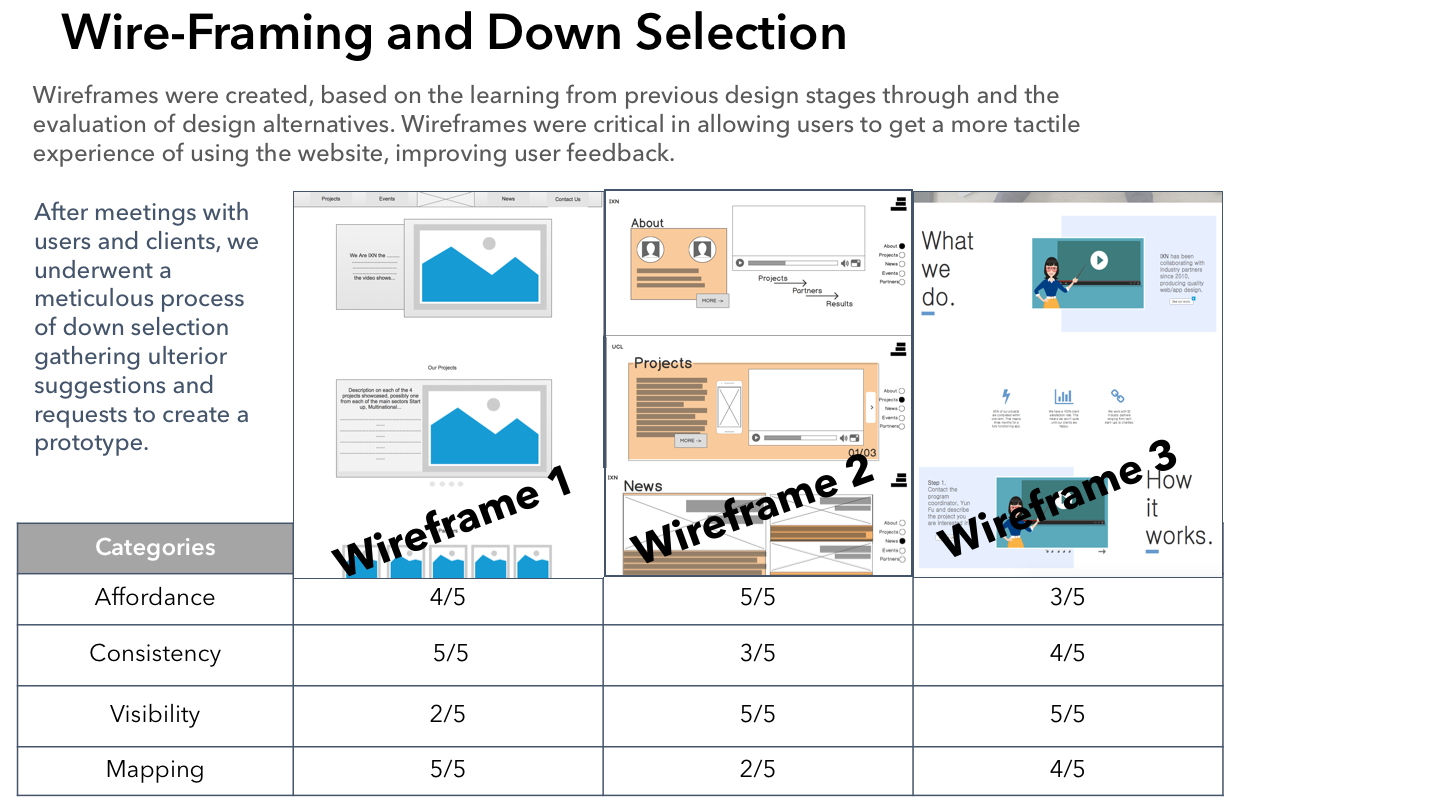
\includegraphics[trim = 0 0 0 0, clip, width=0.99\textwidth]{app1.png}
      \caption{Down selection of wire-frames.}
 \end{figure}
 \end{landscape}

 \begin{landscape}
\subsection{IXN Poll}
\begin{figure}[H]
      \centering
      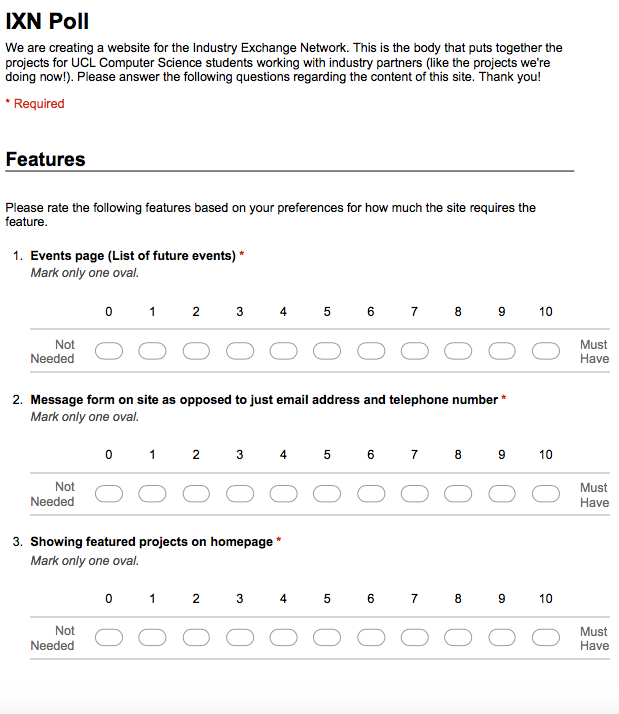
\includegraphics[trim = 0 0 0 0, clip, width=0.99\textwidth]{Poll1.png}
      \caption{IXN poll example page 1. }
 \end{figure}

 \begin{figure}[H]
      \centering
      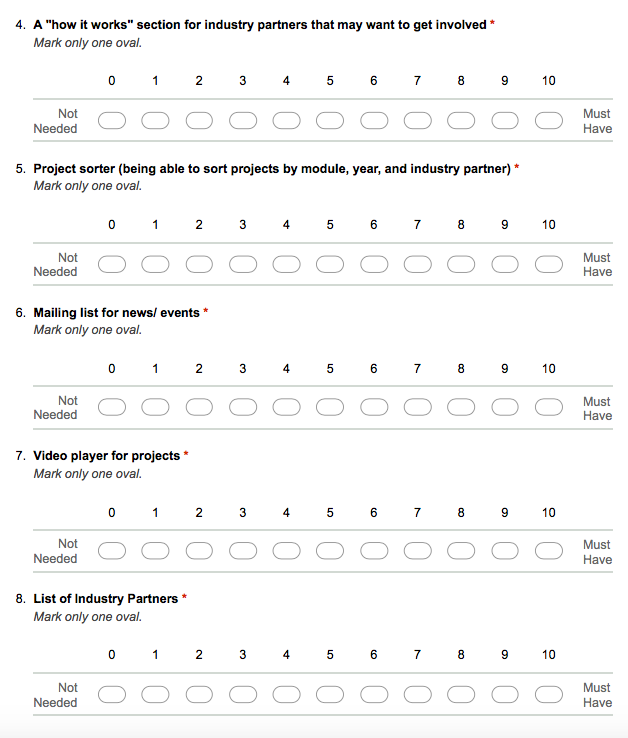
\includegraphics[trim = 0 0 0 0, clip, width=0.99\textwidth]{Poll2.png}
      \caption{IXN poll example page 2.}
 \end{figure}

 \begin{figure}[H]
      \centering
      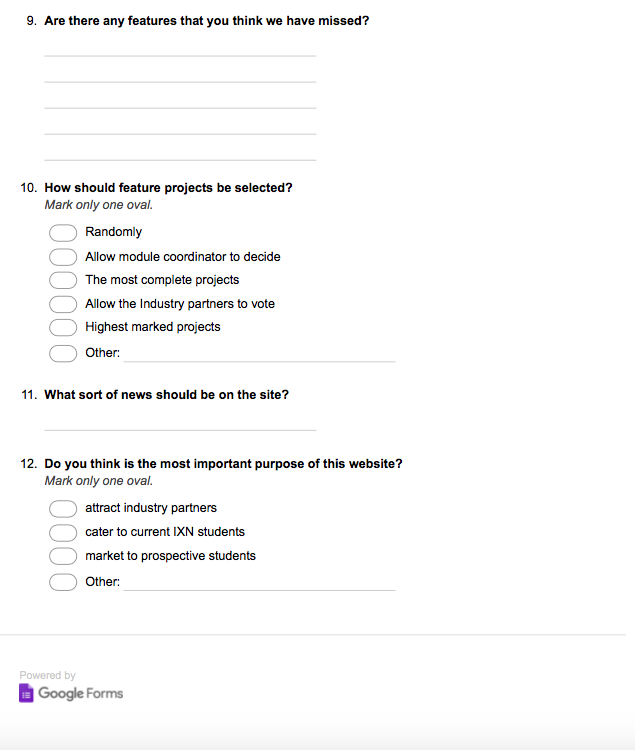
\includegraphics[trim = 0 0 0 0, clip, width=0.99\textwidth]{Poll3.png}
      \caption{IXN poll example page 3.}
 \end{figure}

 \end{landscape}

 \begin{landscape}
\subsection{IXN-Poll-Results}
\begin{figure}[H]
      \centering
      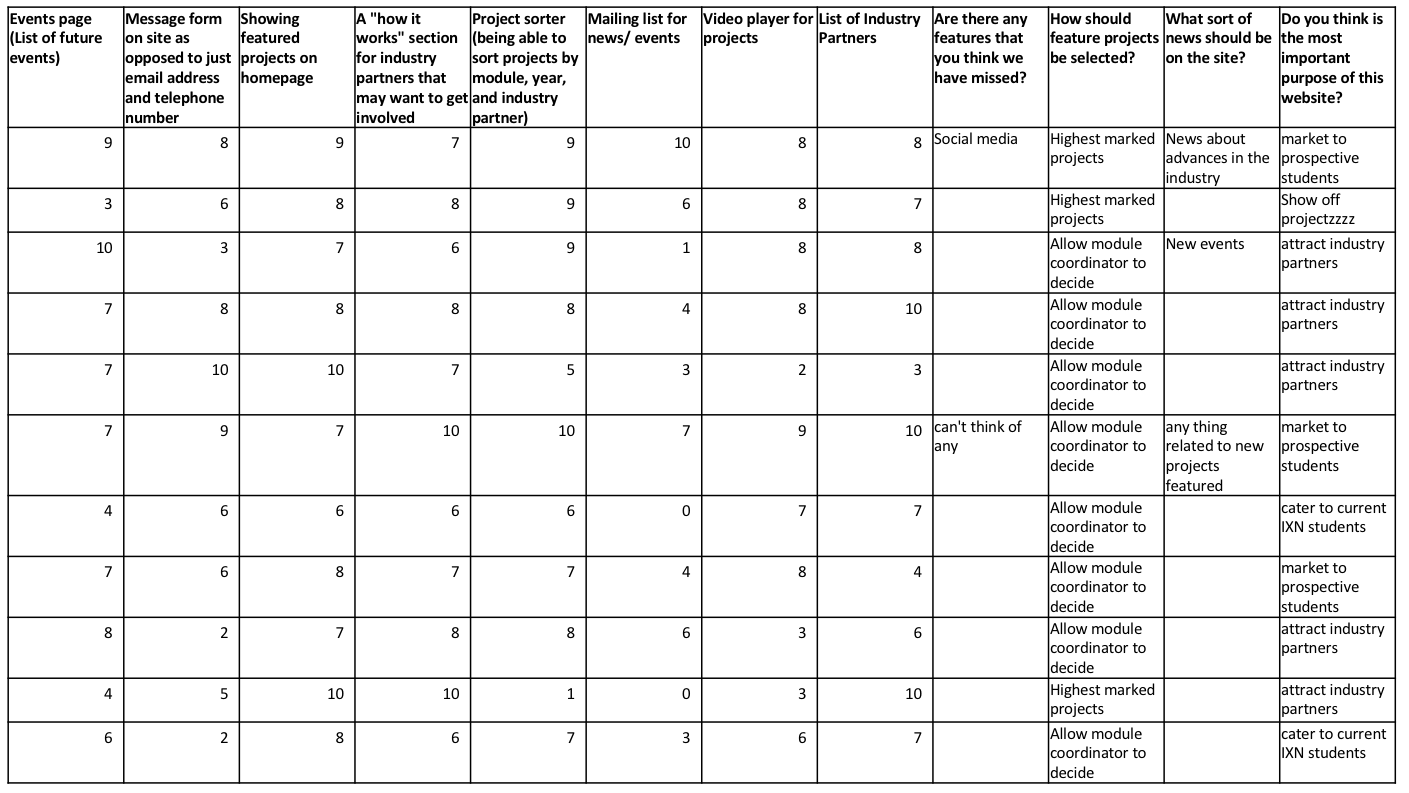
\includegraphics[trim = 0 0 0 0, clip, width=0.99\textwidth]{PollResults.png}
      \caption{Down selection of wire-frames.}
 \end{figure}
 \end{landscape}


\end{document}